\documentclass[12pt,oneside, titlepage]{book}
\usepackage[ngerman]{babel}
\usepackage[utf8]{inputenc}
\usepackage[hidelinks]{hyperref}
\usepackage{inconsolata}
\usepackage{color}
\usepackage{enumitem}
\usepackage{graphicx}
\graphicspath{ {./img/} }
\usepackage[a4paper, left=2.5cm, right=2.5cm, top=2.5cm]{geometry}
\usepackage[onehalfspacing]{setspace}
\usepackage{listings}
\usepackage[pagestyles]{titlesec}   

\newpagestyle{defaultstyle}{\setfoot[\thepage][][]{}{}{\thepage}\sethead[\chaptertitle][][]{}{}{\chaptertitle}}
\pagestyle{defaultstyle}

\definecolor{pblue}{rgb}{0.13,0.13,1}
\definecolor{pgreen}{rgb}{0,0.5,0}
\definecolor{pred}{rgb}{0.9,0,0}
\definecolor{pgrey}{rgb}{0.46,0.45,0.48}

\usepackage{listings}
\lstset{language=Java,
  showspaces=false,
  showtabs=false,
  breaklines=true,
  showstringspaces=false,
  breakatwhitespace=true,
  commentstyle=\color{pgreen},
  keywordstyle=\color{pblue},
  stringstyle=\color{pred},
  basicstyle=\ttfamily,
  moredelim=[il][\textcolor{pgrey}]{$$},
  moredelim=[is][\textcolor{pgrey}]{\%\%}{\%\%}
}


\title{Dokumentation Programmentwurf \\ Vorlesung Advanced Software Engineering \\ DHBW Karlsruhe Semester 5/6}
\author{Lukas Panni \\ TINF18B5}
\begin{document}

\maketitle
\tableofcontents

\documentclass[12pt]{article}
\usepackage[ngerman]{babel}
\usepackage[utf8]{inputenc}
\usepackage[hidelinks]{hyperref}
\usepackage{inconsolata}
\usepackage{color}
\usepackage{enumitem}
\usepackage[a4paper, left=2.5cm, right=2.5cm, top=2.5cm]{geometry}
\usepackage[onehalfspacing]{setspace}


\definecolor{pblue}{rgb}{0.13,0.13,1}
\definecolor{pgreen}{rgb}{0,0.5,0}
\definecolor{pred}{rgb}{0.9,0,0}
\definecolor{pgrey}{rgb}{0.46,0.45,0.48}

\usepackage{listings}
\lstset{language=Java,
  showspaces=false,
  showtabs=false,
  breaklines=true,
  showstringspaces=false,
  breakatwhitespace=true,
  commentstyle=\color{pgreen},
  keywordstyle=\color{pblue},
  stringstyle=\color{pred},
  basicstyle=\ttfamily,
  moredelim=[il][\textcolor{pgrey}]{$$},
  moredelim=[is][\textcolor{pgrey}]{\%\%}{\%\%}
}

\title{Legacy Code}
\date{DHBW Karlsruhe\\ Vorlesung Advanced Software Engineering Semester 5/6}
\author{Lukas Panni \\ TINF18B5}
\begin{document}
\maketitle

\newpage

\tableofcontents

\newpage

\section{Abhängigkeiten brechen}

Im folgenden sollen einige Beispiele aufgeführt werden, bei denen Abhängigkeiten mithilfe der in der Vorlesung behandelten Techniken beseitigt werden.
Ohne diese Abhängigkeiten sind Tests leichter zu entwickeln, sodass weitere Änderungen, zum Beispiel zur Verbesserung des Designs, später einfacher und komfortabler möglich sind.
Das Ziel beim Brechen der Abhängigkeiten ist es, die Testbarkeit der betroffenen Klassen beziehungsweise Methoden zu erhöhen.

\newpage

\subsection{ExtractInterface bei Commit \href{https://github.com/lukaspanni/OpenSourceStats/commit/1e47e7b2d42c04429a433a6ac3dbea781409d36d} {1e47e7b}}
\label{sec:ExtractInterface_AuthHandler_1}

\subsubsection*{\href{https://github.com/lukaspanni/OpenSourceStats/tree/0daf8862a81a976e3d6341f5b5461bc8d3c64b4f/app/src/main/java/de/lukaspanni/opensourcestats/auth/}{Ausgangszustand}}

Die Klasse \textit{AuthHandler} ist stark abhängig von der Android-Klasse \textit{Activity} und kann auch nicht erstellt werden ohne eine Instanz dieser Klasse der \textit{getInstance}-Methode zu übergeben.
Die Testbarkeit ist schlecht, da eine Android-\textit{Activity}-Instanz nicht ohne weiteres im Test-Kontext erstellt werden kann.
Auch ein Fake-Objekt ist schwer zu erstellen, da eine finale Methode genutzt wird, in Ableitungen von \textit{Activity} nicht überschrieben werden kann.
Da die Klasse \textit{AuthHandler} für die OAuth-Authentifizierung verantwortlich ist und damit wichtig für das Gesamtsystem, ist es wichtig, Tests für diese Klasse zu ermöglichen.

\subsubsection*{Gewählte Technik}

Die \textit{getInstance}-Methode benötigt eine Instanz der Klasse \textit{Activity}, die im Test-Kontext nicht leicht erstellbar ist und für die auch Fake-Objekte nur schwer erstellt werden können. Da allerdings nur wenige Methoden der \textit{Activity}-Klasse verwendet werden, und eine Änderung der \textit{AuthHandler} Klasse nur vergleichsweise wenige Änderungen erfordert, kann in diesem Fall \textbf{ExtractInterface} angewendet werden.
So wird die Abhängigkeit von \textit{AuthHandler} zu \textit{Activity} gelöst, indem das Interface \textit{AuthHandlerActivity} eingeführt und der Parameter von \textit{getInstance} angepasst wird, sodass eine Instanz vom Typ des Interfaces verwendet wird. Dabei werden auch kleinere Anpassungen an Methodenaufrufen vorgenommen, sodass Methoden des Interfaces aufgerufen werden.
\textbf{ExtractInterface} ist durch IDE-Unterstützung vergleichsweise einfach und ohne große Fehleranfälligkeit durchzuführen. Außerdem wird die Abstraktion durch diese Technik verbessert.

\subsubsection*{\href{https://github.com/lukaspanni/OpenSourceStats/tree/1e47e7b2d42c04429a433a6ac3dbea781409d36d/app/src/main/java/de/lukaspanni/opensourcestats/auth/}{Endzustand}}

\textit{AuthHandler} nutzt nach dieser Änderung nur noch die Methoden des Interfaces, wodurch die Testbarkeit erhöht wird.
Allerdings gibt es hier das Problem, dass \textit{AuthHandler} die Third-Party-Klasse \textit{AuthorizationService} verwendet, die auf eine \textit{Activity}-Instanz angewiesen ist.
Deshalb gibt es im neu eingeführten Interface eine Methode, die eine \textit{Activity} zurückgibt. Die Abhängigkeit konnte also in diesem Fall nicht komplett aufgelöst werden.
Trotzdem wurde die Testbarkeit erhöht und die Abstraktion verbessert. Diese Änderung stellt damit eine gute Basis für weitere Refactorings und Änderungen dar, wie zum Beispiel in Commit \href{https://github.com/lukaspanni/OpenSourceStats/commit/cbc53183a878d6507a02daebd55c9c7dfcae9c0f}{cbc5318}.

\newpage

\subsection{Parametrize Constructor bei Commit \href{https://github.com/lukaspanni/OpenSourceStats/commit/d098b93ffd042cb095af679254ed01584417763e} {d098b93}}

\subsubsection*{\href{https://github.com/lukaspanni/OpenSourceStats/tree/3b1eb5bf6750c3ccaeb05962ec8a8ae743adbf2c/app/src/main/java/de/lukaspanni/opensourcestats/repository}{Ausgangszustand}}

Die Klassen \textit{RepositoryDataRepository} und \textit{UserContributionsRepository} haben eine Abhängigkeit zur Klasse \textit{ResponseCache} und erzeugen im Konstruktor eine Instanz dieser Klasse und speichern diese in einer Instanzvariablen.
Für den Test der Klassen ist es hilfreich, diese Instanzvariable durch eine eigene Cache-Implementierung zu nutzen.
In diesem Fall lässt sich die Abhängigkeit mit Hilfe von \textbf{Parametrize Constructor} brechen.
\newline
Dazu wird ein neuer Konstruktor erzeugt, der einen zusätzlichen Parameter vom Typ der zu überschreibenden Instanzvariable entgegennimmt. In diesem Beispiel eine Instanz von \textit{ResponseCache}. Die existierenden Konstruktoren rufen den neuen Konstruktor mit dem ursprünglichen Wert der Variable auf.
Dabei bleibt die alte Funktionalität erhalten und es müssen keine Anpassungen an anderen Stellen erfolgen.

\subsubsection*{\href{https://github.com/lukaspanni/OpenSourceStats/tree/d098b93ffd042cb095af679254ed01584417763e/app/src/main/java/de/lukaspanni/opensourcestats/repository}{Endzustand}}

Durch das Brechen der Abhängigkeit ist es nun möglich, beim Erstellen einer Instanz vom Typ \textit{RepositoryDataRepository} oder \textit{UserContributionsRepository} ein \textit{ResponseCache}-Objekt zu übergeben. Dadurch kann zum Beispiel beim Test ein Fake-Objekt übergeben werden.
\newpage


\subsection{ExtractInterface bei Commit \href{https://github.com/lukaspanni/OpenSourceStats/commit/da964f5d7e2485f28cf19b4ec178b92805538adc} {da964f5}}
\label{sec:ExtractInterface_AuthHandler_2}

\subsubsection*{\href{https://github.com/lukaspanni/OpenSourceStats/tree/473384cdb4bc8e9f8269af865cf210923c42b5c5/app/src/main/java/de/lukaspanni/opensourcestats/auth}{Ausgangszustand}}

Ein Objekt der Klasse \textit{AuthHandler} wird zum Beispiel in der Klasse \textit{GHClient} (bei da964f5 umbenannt in \textit{GithubOAuthClient}) benötigt, um Daten über die API abrufen zu können. Aktuell ist ein Test dieser Komponente nur schwer möglich, da \textit{AuthHandler} selbst wiederum Abhängigkeiten zu einer Third-Party Bibliothek besitzt. Deshalb ist hier das erstellen von Fake-/Mock-Objekten sehr aufwändig. Bei \ref{sec:ExtractInterface_AuthHandler_1} wurde bereits die Testbarkeit der \textit{AuthHandler}-Klasse erhöht und durch ExtractInterface an dieser Stelle soll die Testbarkeit der von \textit{AuthHandler} abhängigen Klassen erhöht werden.

\subsubsection*{Gewählte Technik}

Es wurde \textbf{ExtractInterface} gewählt um Abhängigkeiten zu \textit{AuthHandler} zu beseitigen. Dazu wurde das Interface \textit{AuthenticationHandler} eingeführt wird, das in der alten \textit{AuthHandler}-Klasse (zur besseren Verständlichkeit umbenannt zu \textit{GithubOAuthHandler}) implementiert wird. 
Um den Vorgang zu ermöglichen wurde zuvor die Singleton-Eigenschaft entfernt (\href{https://github.com/lukaspanni/OpenSourceStats/commit/13efee847af5b7627391d2ae6309b800727c51fd}{13efee8}) und die Methoden und ihre Verwender wurden angepasst (\href{https://github.com/lukaspanni/OpenSourceStats/commit/473384cdb4bc8e9f8269af865cf210923c42b5c5}{473384c}). 
Anschließend kann das Interface erstellt werden und bei allen Verwendern der Ursprünglichen Klasse, die dies erlauben, die Abhängigkeit zur Konkreten Klasse durch eine Abhängigkeit zum Interface ersetzt werden.

\subsubsection*{\href{https://github.com/lukaspanni/OpenSourceStats/tree/da964f5d7e2485f28cf19b4ec178b92805538adc/app/src/main/java/de/lukaspanni/opensourcestats/auth}{Endzustand}}

In der Klasse \textit{GithubOAuthClient} konnte die Abhängigkeit zu \textit{GithubOAuthHandler} (vormals \textit{AuthHandler} vollständig beseitigt werden.
 Dadurch werden Tests der Klasse mit Fake-/Mock-Implementierungen des neuen Interfaces \textit{AuthenticationHandler} möglich. 
Außerdem wird die Abstraktion verbessert und die konkrete Authentifizierungs-Klasse könnte leichter ausgetauscht werden, was zum Beispiel benötigt wird, wenn ein anderes OAuth-Framework eingesetzt werden sollte.

\newpage

\subsection{Parametrize Method bei Commit \href{https://github.com/lukaspanni/OpenSourceStats/commit/d8c995c387a792a6d83c852119760b0c57a63c02} {d8c995c}}

\subsubsection*{\href{https://github.com/lukaspanni/OpenSourceStats/tree/eafe840d0bfc8a08beca01709003d5afe7e59963/app/src/main/java/de/lukaspanni/opensourcestats/util/TimeSpanFactory.java}{Ausgangszustand}}
Die Klasse \textit{TimeSpanFactory}, die verwendet wird um \textit{TimeSpan}-Objekte zu erzeugen hat eine starke Abhängigkeit zur Java-Klasse \textit{java.util.Calendar}.
In den Methoden von TimeSpanFactory wird jeweils eine Calendar-Instanz benötigt. 
Um diese zu erhalten wird die Methode \textit{Calendar.getInstance()} verwendet.
Da die verwendete Calendar-Instanz das Ergebnis der Methoden beeinflusst muss die Instanz für Tests ausgetauscht werden können.
Dies ist aber aktuell nicht möglich.

\subsubsection*{Gewählte Technik}
Um die Abhängigkeit der Methoden zu \textit{Java.util.Calendar} zu beseitigen wurde die Technik \textbf{Parametrize Method} gewählt.
Bei dieser Technik wird für die Methode, bei der die Abhängigkeit gebrochen werden muss, eine neue Methode mit einem zusätzlichen Parameter angelegt.
Dieser Parameter ersetzt dann die Variable, die im Test benötigt wird.
Die eigentliche Funktionalität der alten Methode wird in die neue Methode verschoben und die alte Methode ruft diese mit dem ursprünglichen Wert der Variablen auf.
So sind keine Änderungen an bestehendem Code notwendig und trotzdem wird ein Test der Methode ermöglicht.

\subsubsection*{\href{https://github.com/lukaspanni/OpenSourceStats/tree/d8c995c387a792a6d83c852119760b0c57a63c02/app/src/main/java/de/lukaspanni/opensourcestats/util/TimeSpanFactory.java}{Endzustand}}

Die Technik Parametrize Method wurde für mehrere Methoden in TimeSpanFactory angewendet um die Abhängigkeit zu lösen, sodass Tests nun möglich sind.
Durch die Möglichkeit eine Calendar-Instanz zu übergeben können die Methoden einfach getestet werden.


\end{document}

\chapter{Refactoring}

\section{Code Smells} 

Im Folgenden sollen bekannte Code Smells im Code identifiziert werden. Im Abschnitt \hyperref[sec:Refactorings]{Refactorings} werden Refactorings beschrieben, die einige der Identifizierten Code Smells beheben sollen.


\subsection{Duplicated Code}
\label{sec:Duplicated_Code}

\textit{Duplicated Code} beschreibt, dass der gleiche beziehungsweise sehr ähnlicher Code an mehreren Stellen des Systems vorkommt.
Dadurch ist der Wartungsaufwand vergleichsweise hoch, da bei jeder Änderung potentiell mehrere Stellen angepasst werden müssen. Das kann auch dazu führen, dass sich die Funktionalität der einzelnen Stellen im Laufe der Zeit minimal unterscheidet, wodurch das Verhalten des Systems inkonsistent wird.
Um Duplicated Code zu reduzieren muss der doppelte Code ausgelagert werden und kann dann an verschiedenen Stellen wiederverwendet werden.
Die folgende Liste enthält Beispiele für Duplicated Code im vorliegenden Projekt.
\begin{itemize}
	\item{TimeSpanDetails: Click-Listener-Code wird vier mal in gleicher Form (bis auf eine Variable) verwendet. Gelöst mit {\hyperref[sec:ExtractMethod_TimeSpanDetails]{ExtractMethod}} bei Commit \href{https://github.com/lukaspanni/OpenSourceStats/commit/0c0b357dee742575d8465ae26e64152bfecbf5ab} {0c0b357}}
	
	\item{\textit{UserContributionRepository.userContributionsTimeSpan} und \textit{RepositoryDataRepository.repositorySummary} sind, bis auf die verwendeten Datentypen sehr ähnlich. 
Da beide Klassen von der gleichen Basisklasse erben wäre die Auslagerung einer Methode, in die Basisklasse eine denkbare Lösung.
\newline
Ein erster Schritt zur Verringerung des doppelten Codes ist durch das Refactoring {\hyperref[sec:ExtractMethod_Repository]{ExtractMethod}} bei Commit \href{https://github.com/lukaspanni/OpenSourceStats/commit/3b1eb5bf6750c3ccaeb05962ec8a8ae743adbf2c} {3b1eb5b} bereits umgesetzt.} 		
\end{itemize}
Ansonsten konnten keine weiteren duplizierten Code-Teile gefunden werden.
Da nur wenige Dopplungen gefunden wurden und nur noch eine Kopplung weiterhin besteht, kann abschließend gesagt werden, dass der Code weitgehend frei von unnötigen Duplizierungen ist.

\subsection{Long Method \& Large Class}

Der Code Smell \textit{Long Method} zeichnet sich durch sehr lange Methoden aus, wobei die Länge, ab der eine Methode als zu lang betrachtet wird, von Projekt zu Projekt variabel sein kann.
Lange Methoden erschweren das Verständnis des Codes, was wiederum die Wartbarkeit und auch die Erweiterbarkeit einschränkt. 
Als Lösung kann die Lange Methode in mehrere kürzere Methoden aufgeteilt werden.
\newline
\newline
Ähnlich wie Long Method beschreibt \textit{Large Class}, Klassen, die vergleichsweise viele Code-Zeilen beinhalten.
Dies kommt häufig vor, wenn mehrere Verantwortlichkeiten in einer Klasse untergebracht werden. Auch hier kann die Verständlichkeit des Codes erschwert werden.
Das Aufteilen der Klasse in mehrere Klassen, ist eine sinnvolle Lösung für diesen Code Smell.
\newline
\newline
Um sowohl lange Methoden als auch große Klassen zu finden wurde das Code-Statistik Plugin \href{https://plugins.jetbrains.com/plugin/4509-statistic}{\textit{Statistic}} für Android Studio verwendet.
Um große Klassen oder Methoden zu finden, muss zunächst eine Obergrenze für die Methodenlänge fesgelegt werden.
Legt man zusätzlich eine maximale Anzahl von Methoden pro Klasse fest, lässt sich eine maximale Klassenlänge ableiten.
Im Buch \textit{Refactoring in Large Software Projects} wird angegeben, dass Methoden im Durchschnitt nicht länger als 30 Zeilen sein sollten \cite[p.~31]{refactoring_lippert}.
Außerdem wird beschrieben, dass eine Klasse weniger als 30 Methoden und damit auch weniger als 900 Zeilen umfassen sollte.
Die Längenvorgabe für Methoden soll auch hier verwendet werden.
Eine Klasse mit 900 Zeilen Code, ist aber meiner Meinung nach zu unübersichtlich für den praktischen Gebrauch.
Stattdessen sollte eine Klasse maximal etwa 200 Zeilen Code umfassen.
So kann der Code der Klasse noch schnell erfasst und verstanden werden und gleichzeitig wird eine zu starke Fragmentierung in viele einzelne Datein vermieden.
Aus diesem Grund sollen alle Klassen kleiner als 200 Zeilen Code sein.
\newline
Abbildung \ref{fig:class_length} zeigt die Länge der längsten Klassen im Projekt.
Keine der Klassen erreicht die maximale Anzahl an Zeilen.
Um die Länge der Methoden festzustellen wurden alle Klassen mit einer Länge von über 30 Zeilen untersucht.
Die Längste gefundene Methode besteht aus 28 Code-Zeilen und ist damit knapp kürzer als erlaubt.
\begin{figure}[h]
  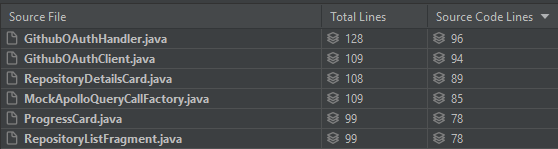
\includegraphics{class_length.png}
  \centering
  \caption{Größte Klassen des Projekts}
  \label{fig:class_length}
\end{figure}

\subsection{Shotgun Surgery}

\textit{Shotgun Surgery} beschreibt, dass für vergleichsweise kleine Funktionale Änderungen Anpassungen an vielen Stellen notwendig sind und deutet auf schlechte Struktur und eine Verflechtung von Verantwortlichkeiten hin.
Durch eine Umstrukturierung des Codes, sodass jede Klasse nur eine Verantwortlichkeit hat, kann dies behoben werden.
\newline
\newline
Dieser Code-Smell ist vergleichsweise schwer zu entdecken, wenn man danach sucht. Stattdessen kann dieser Code-Smell bei Anpassungen des Codes entdeckt werden.
Bisher wurde dieser Code-Smell bei keiner Änderung entdeckt.

\subsection{Switch Statements}

Die Verwendung von \textit{Switch Statements} fördert Fehler durch die unintuitive Syntax und verleitet oft dazu das gleiche Switch-Statement an mehreren Stellen einzusetzen.
Durch das übermäßige Verwenden von Switch Statements wird die Wartbarkeit und auch die Erweiterbarkeit des Codes eingeschränkt.
Switch Statements können in Objektorientiertem Code häufig durch die Verwendung von Polymorphie reduziert werden.
\newline
\newline
Im gesamten Code konnten keine Switch-Statements entdeckt werden. Außerdem wurde auch das Alternativkonstrukt (lange if-else Verkettungen) nicht entdeckt.

\subsection{Code Comments}

\textit{Code Comments} die beschreiben, was der Code an dieser Stelle tut, deuten häufig darauf hin, dass der Code an dieser Stelle unverständlich geschrieben ist.
\newline
\newline
Durch die Suche nach Kommentaren und eine Beurteilung der Kommentare in Bezug auf diesen Code-Smell ergab den folgenden Kommentar in den Klassen \textit{UserContributionsRepository} und \textit{RepositoryDataRepository}, der beschreibt, was der Code an dieser Stelle tut, was auf unverständlichen Code hindeutet.
\begin{lstlisting}
//Wrap callback to add response to cache
ClientDataCallback decoratedCallback = new ClientDataCallbackDecorator(callback, response ->  cache.put(repository, response));
\end{lstlisting}
Der Code an dieser Stelle ist ohne den Kommentar schwer verständlich. Um die Verständlichkeit des Codes zu erhöhen wurde das Refactoring {\hyperref[sec:ExtractMethod_Repository]{ExtractMethod}} bei Commit \href{https://github.com/lukaspanni/OpenSourceStats/commit/3b1eb5bf6750c3ccaeb05962ec8a8ae743adbf2c} {3b1eb5b} angewendet und die extrahierte Methode in die Basisklasse verschoben.


\newpage
\section{Refactorings}
\label{sec:Refactorings}

Die hier beschriebenen Refactorings sollen das Design des Systems verbessern, die Wartbarkeit und Erweiterbarkeit verbessern und auch die Verständlichkeit erhöhen.
Dadurch soll es unter anderem einfacher werden Fehler zu finden und zu beheben sowie neue Funktionen hinzuzufügen.


\subsection{ExtractMethod bei Commit \href{https://github.com/lukaspanni/OpenSourceStats/commit/0c0b357dee742575d8465ae26e64152bfecbf5ab} {0c0b357}}
\label{sec:ExtractMethod_TimeSpanDetails}

In der Klasse \textit{TimeSpanDetails} wurde sehr ähnlicher Code für einen Click-Listener an vier unterschiedlichen Stellen verwendet. Durch die Auslagerung in die Methode \textit{getClickListener}  kann der Duplicated Code vermieden werden. Durch die Einführung des Parameters \textit{resource} kann die extrahierte Methode flexibel an allen Stellen wiederverwendet werden. Dadurch wird außerdem die Lesbarkeit des Codes erhöht.
Auch eventuelle spätere Änderungen am Verhalten der Methode müssen so nur an einer Stelle durchgeführt werden.
\newline
\textbf{Code Vorher:} 
\begin{lstlisting}[breaklines=false]
[...]
view.findViewById(R.id.to_commit_repos)
    .setOnClickListener(v -> Navigation.findNavController(view)
    .navigate(R.id.action_1, getArguments()));
view.findViewById(R.id.to_issue_repos)
    .setOnClickListener(v -> Navigation.findNavController(view)
    .navigate(R.id.action_2, getArguments()));
[...]
\end{lstlisting}
\textbf{Code Nacher:} 
\begin{lstlisting}[breaklines=false]
[...]
view.findViewById(R.id.to_commit_repos)
    .setOnClickListener(getClickListener(view, R.id.action_1));
view.findViewById(R.id.to_issue_repos)
    .setOnClickListener(getClickListener(view, R.id.action_2));
[...]
\end{lstlisting}

\newpage
\subsection{ExtractMethod bei Commit \href{https://github.com/lukaspanni/OpenSourceStats/commit/3b1eb5bf6750c3ccaeb05962ec8a8ae743adbf2c} {3b1eb5b}}
\label{sec:ExtractMethod_Repository}

In den Klassen \textit{UserContributionsRepository} und \textit{RepositoryDataRepository} wurde doppelter und zusätzlich schlecht verständlicher Code verwendet. Um die Verständlichkeit des Codes zu erhöhen wurde eine Methode extrahiert und so benannt, dass die Funktion leicht verständlich ist. Die extrahierte Methode wurde in die Basisklasse verschoben, da diese Methode in allen Ableitungen der Basisklasse verwendet wird. Diese Änderung ist vergleichsweise klein erhöht jedoch die subjektive Verständlichkeit enorm.
\subsubsection*{Code Vorher:}
\begin{lstlisting}[breaklines=false]
ClientDataCallback decoratedCallback = new ClientDataCallbackDecorator(
	callback, 
	response -> cache.put(
		repository, (RepositoryDataResponse) response));
\end{lstlisting}
\subsubsection*{Code Nacher:}
\begin{lstlisting}[breaklines=false]
ClientDataCallback decoratedCallback = new ClientDataCallbackDecorator(
	callback, 
	getAddToCacheCallback(repository));
\end{lstlisting}

\newpage
\subsubsection{UML Vorher}
Abbildung \ref{fig:ExtractMethod_Refactoring_Before} zeigt das UML-Klassendiagramm vor dem Refactoring.
\begin{figure}[h]
  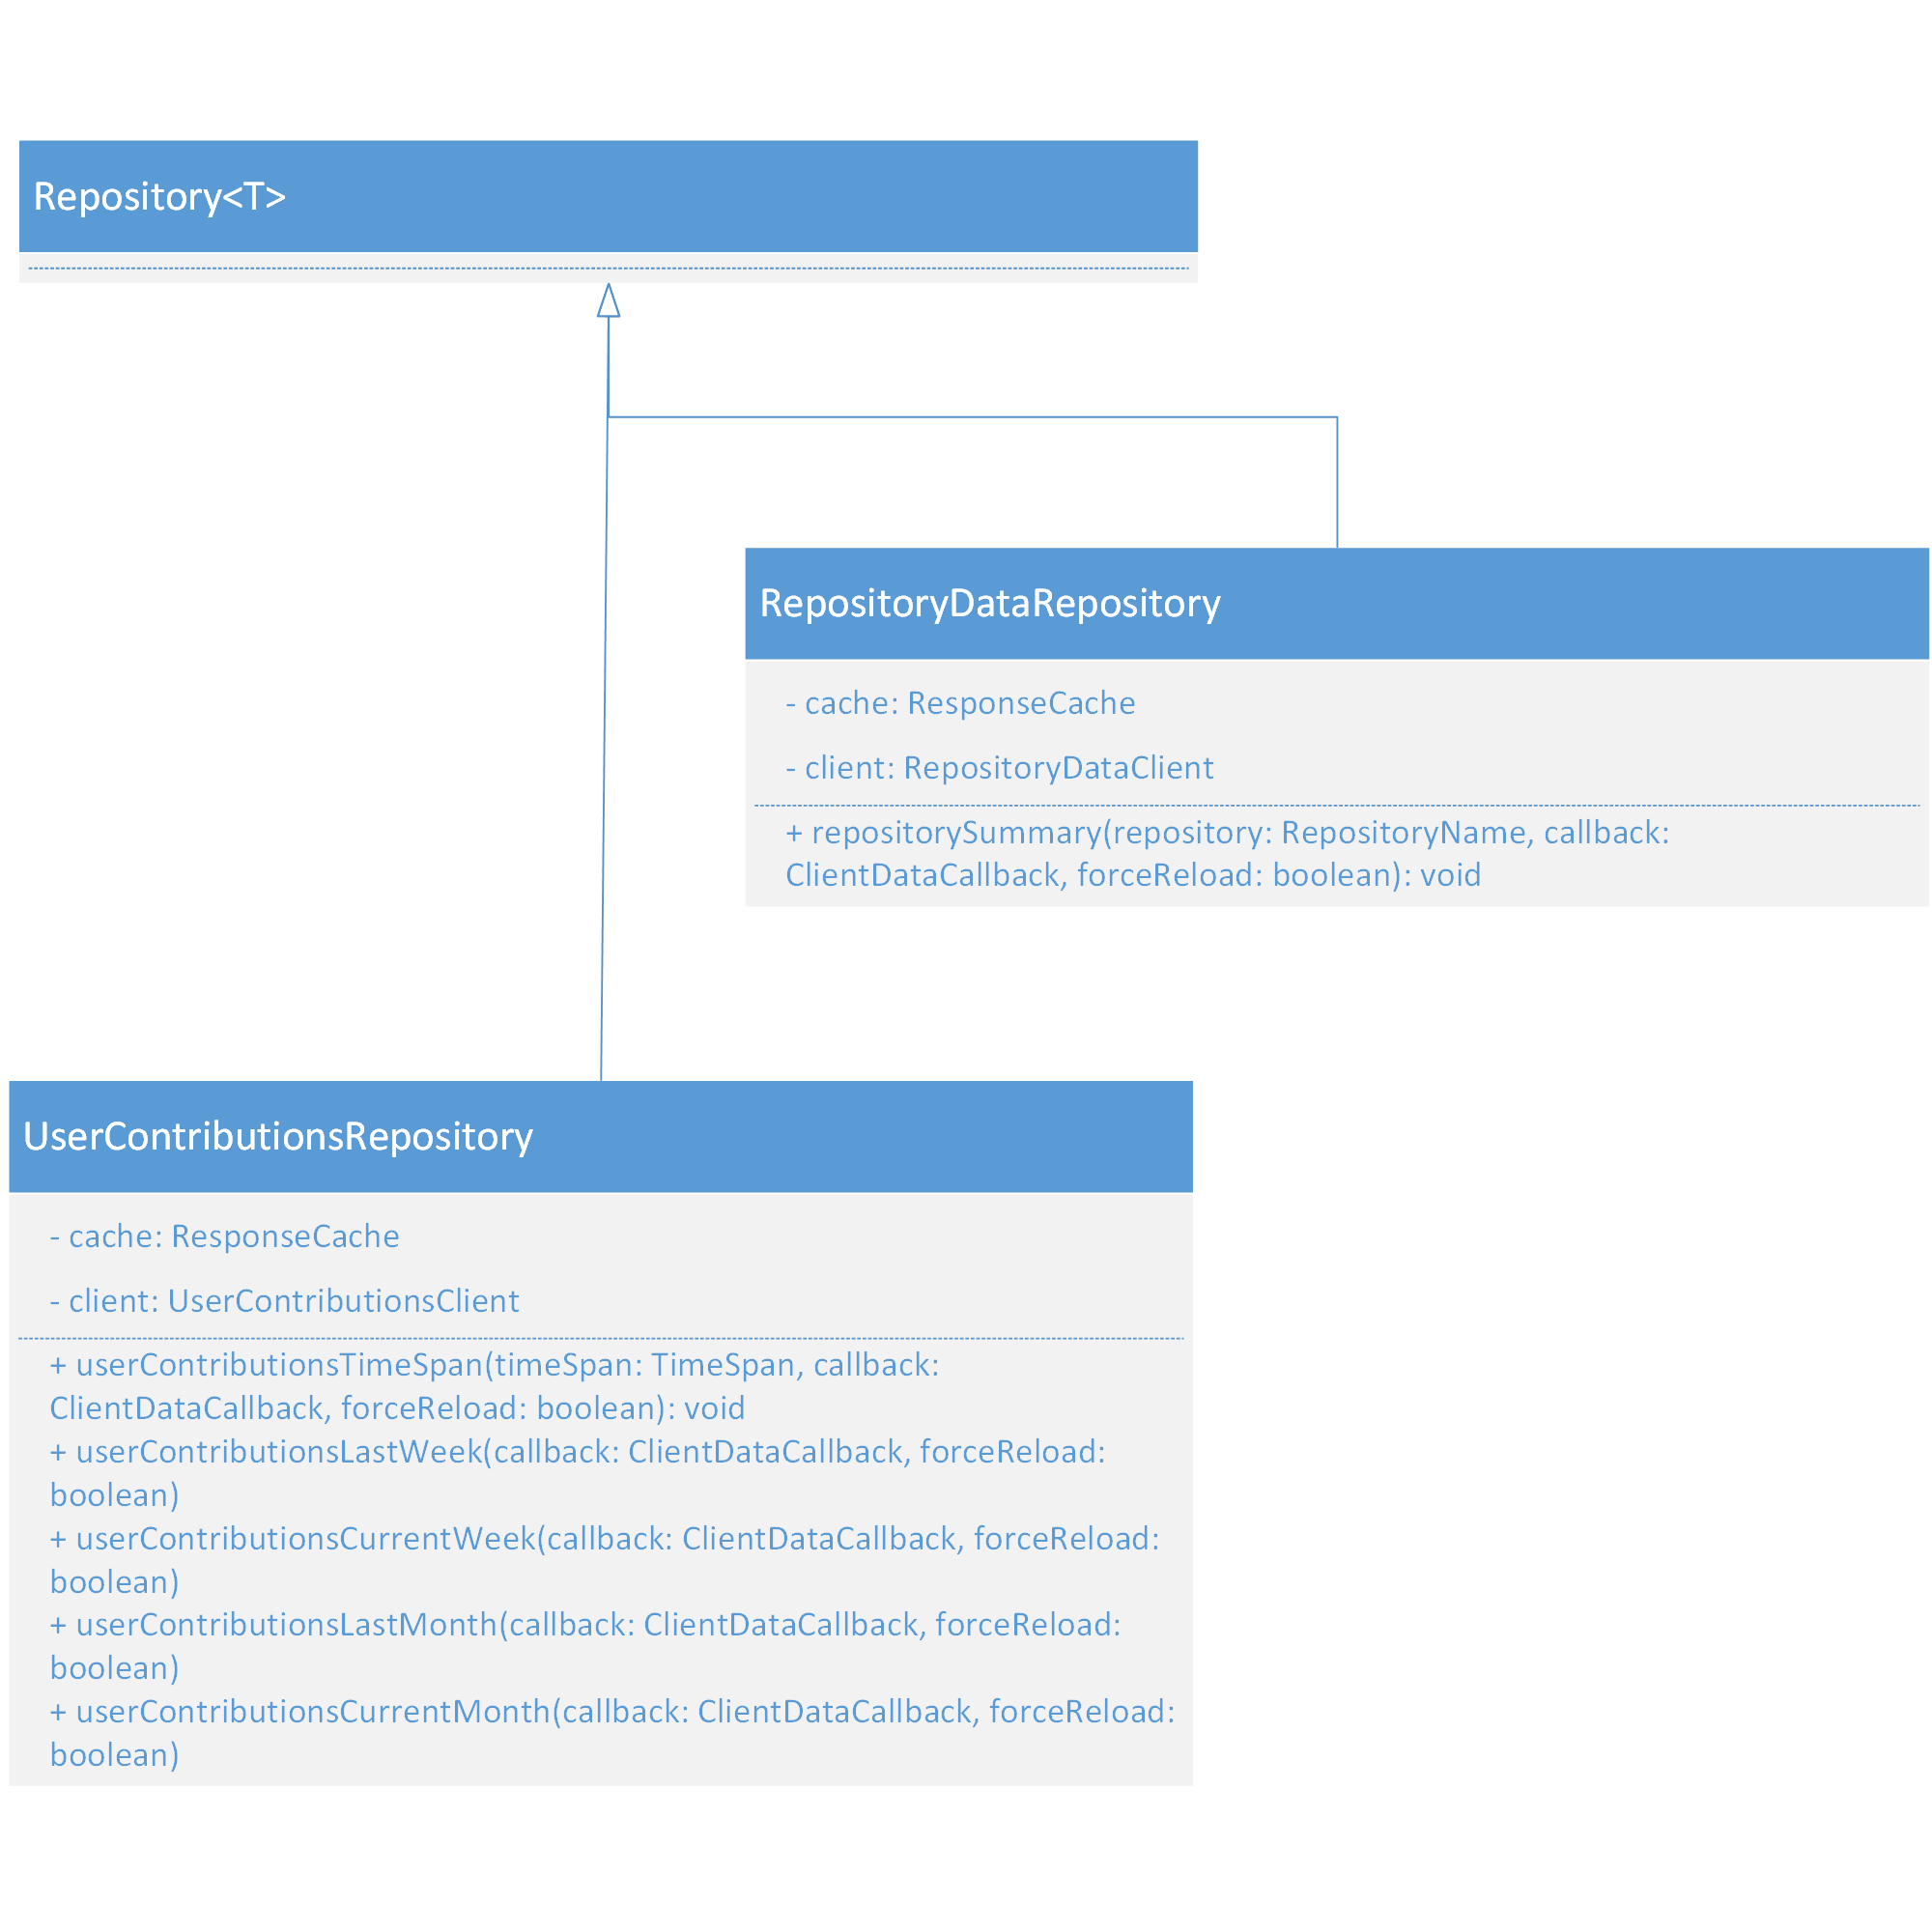
\includegraphics{refactoring_extract_method_repository_before.png}
  \centering
  \caption{UML vor Refactoring}
  \label{fig:ExtractMethod_Refactoring_Before}
\end{figure}

\newpage
\subsubsection{UML Nacher}
Abbildung \ref{fig:ExtractMethod_Refactoring_After} zeigt das UML-Klassendiagramm nach dem Refactoring.
\begin{figure}[h]
  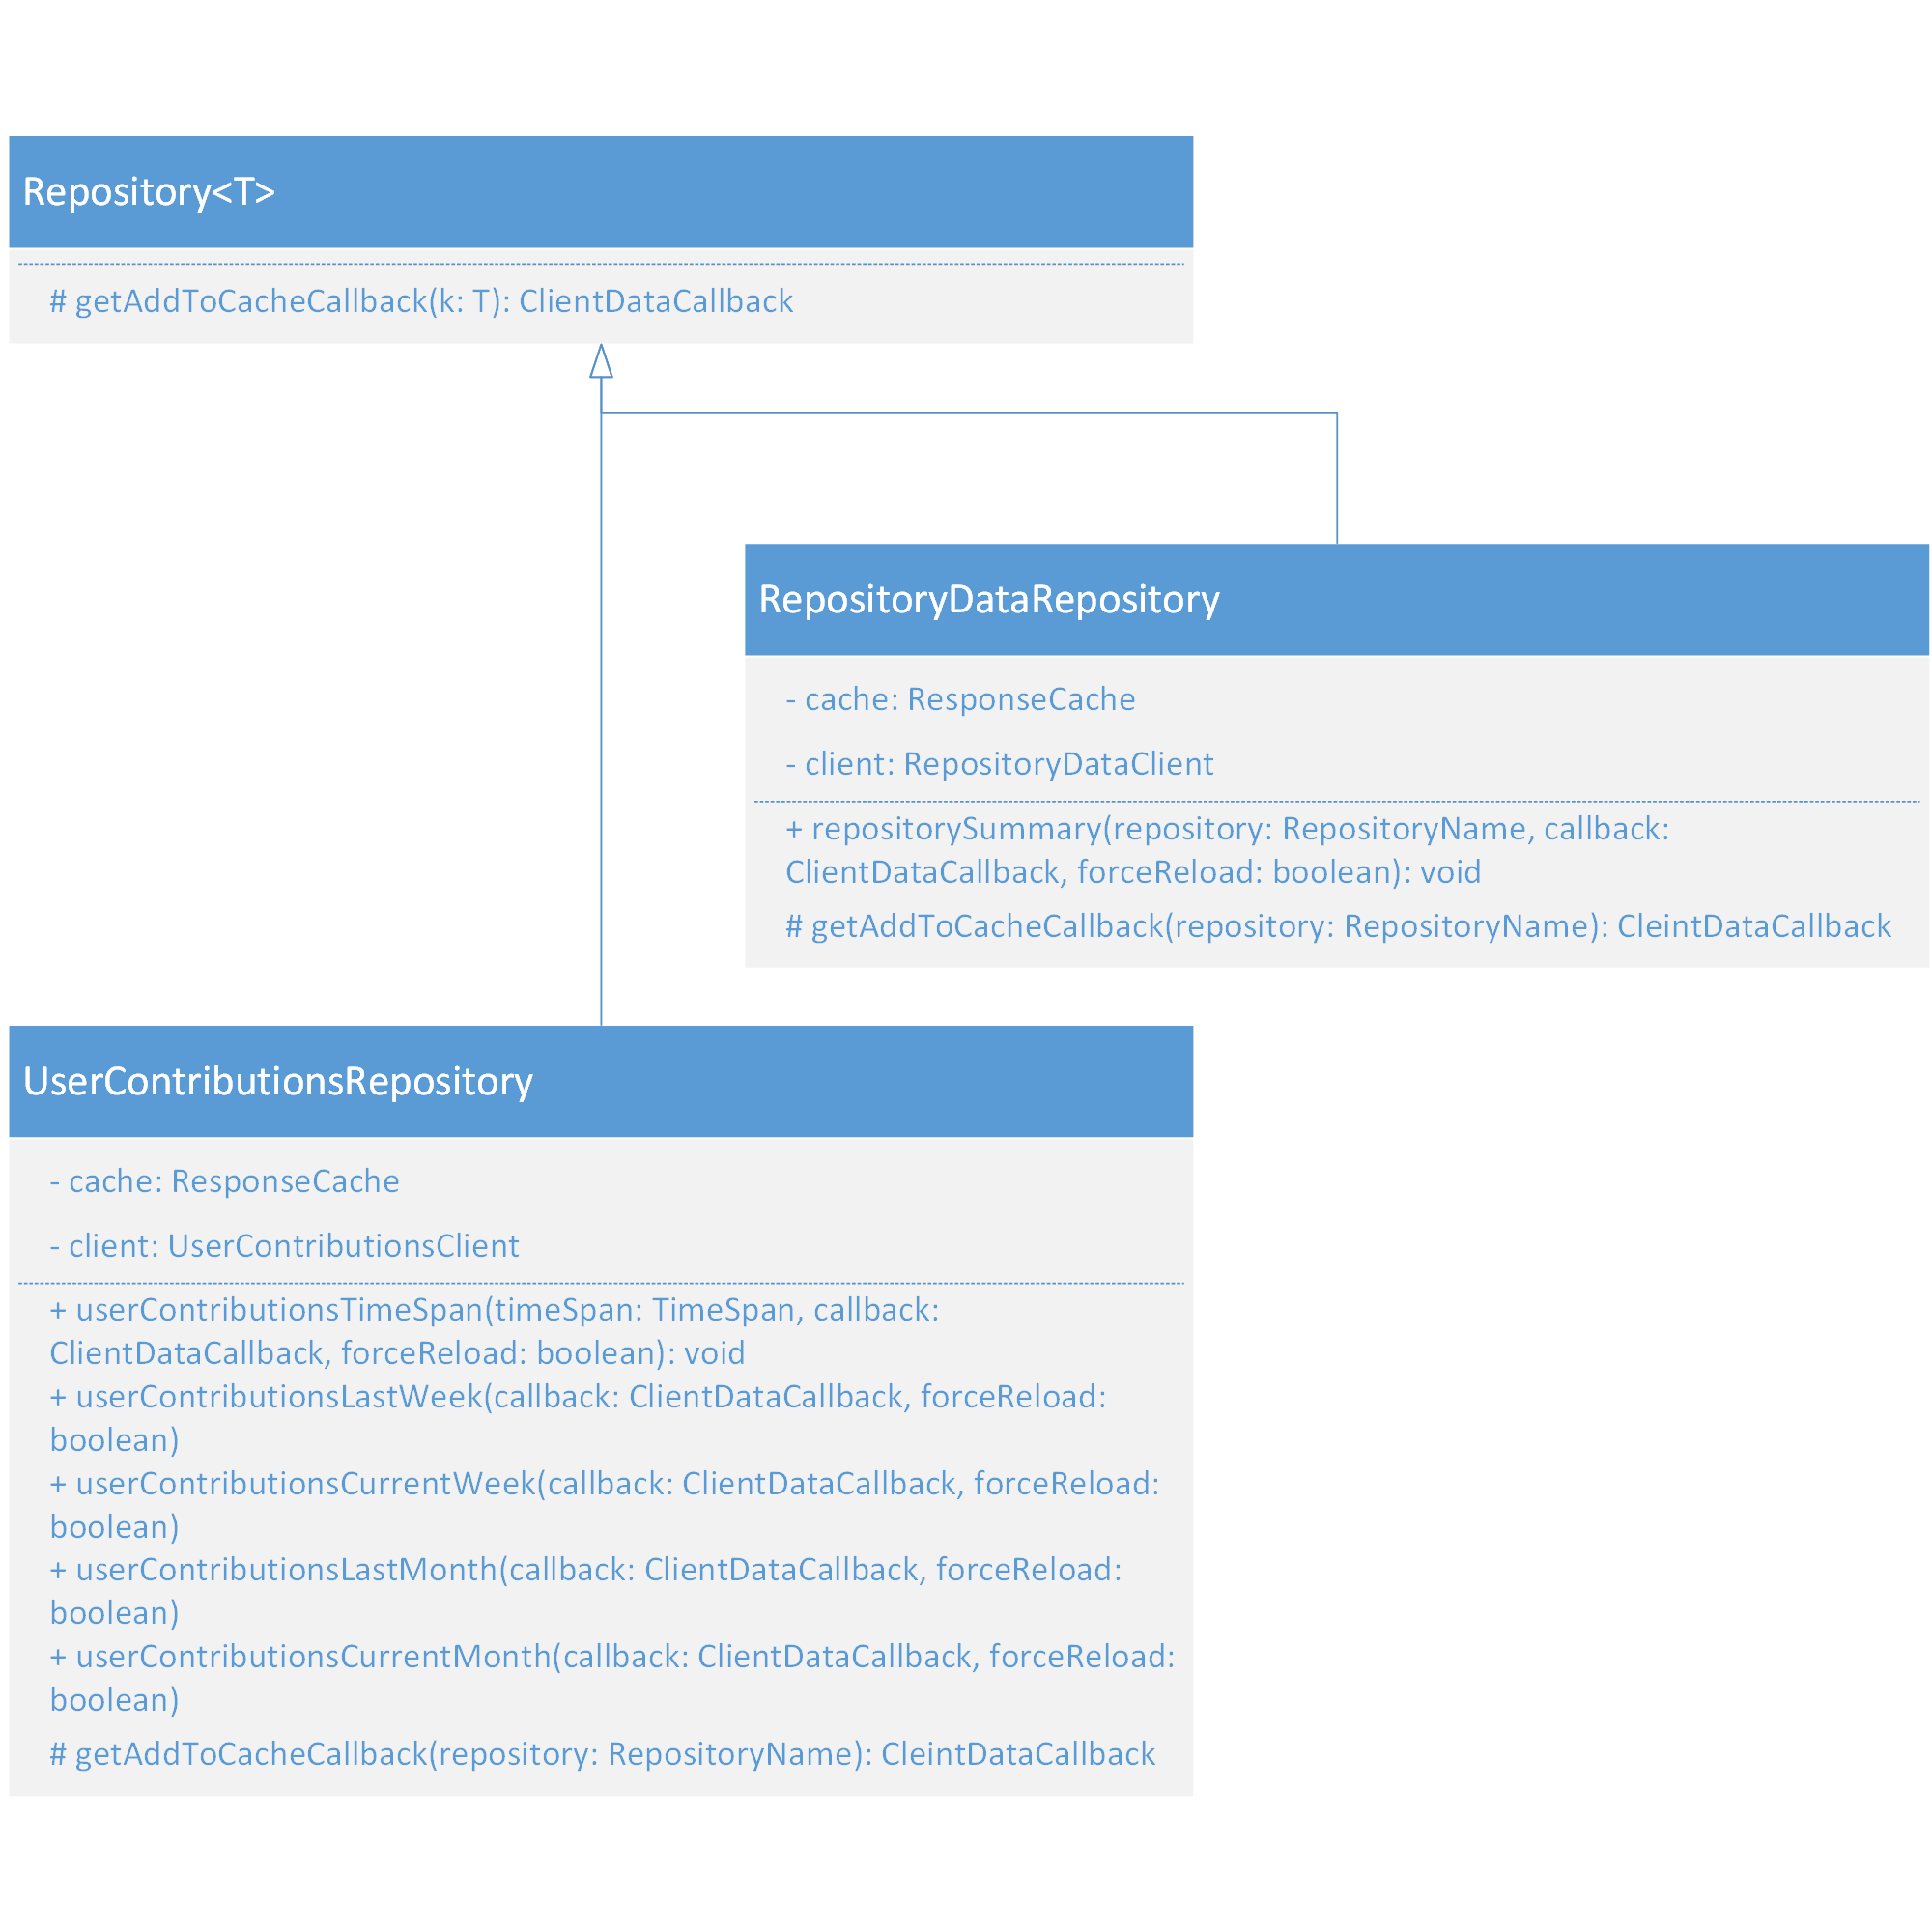
\includegraphics{refactoring_extract_method_repository_after.png}
  \caption{UML nach Refactoring}
  \label{fig:ExtractMethod_Refactoring_After}
\end{figure}
\newpage


\subsection{ExtractMethod bei Commit \href{https://github.com/lukaspanni/OpenSourceStats/commit/2eedf85be90e2566aa3811f9ccd3bac860c444a2} {2eedf85}}
\label{sec:ExtractMethod_AuthHandler}

Um die Singleton-Eigenschaft der Klasse \textit{AuthHandler} entfernen zu können, muss ein Teil der \textit{getInstance()} Methode in eine andere Methode übertragen werden.
Dafür wird das Refactoring \textbf{ExtractMethod} angewendet. So kann kann das Verhalten wiederverwendet werden. Teile des Verhaltens der \textit{getInstance()} Methode sind dadurch noch erhalten, auch wenn die ursprüngliche Methode in einem späteren Commit entfernt wird.


\subsection{RenameMethod bei Commit \href{https://github.com/lukaspanni/OpenSourceStats/commit/650235a5868f35cd0c641f0112b921ddead17a17} {650235a}}
\label{sec:RenameMethod_Repositories}

In den beiden Klassen \textit{RepositoryDataRepository} und \textit{UserContributionsRepository} werden Methodennamen verwendet, die den Zweck der Methode nur schwer verständlich machen. Um dies zu beheben wurde das Refactoring \textbf{ExtractMethod} angewendet.
\subsubsection*{RepositoryDataRepository}
Die Methode \textit{RepositoryDataRepository.repositorySummary} wurde umbenannt in \textit{RepositoryDataRepository.loadRepositoryData}, da dieser Name die Funktion der Methode deutlich besser beschreibt. Der alte Methodenname beschreibt nur den Zusammenhang mit einer Zusammenfassung über ein Repository, zeigt aber nicht deutlich genug, dass in dieser Methode Daten zu einem übergebenen Repository geladen werden. Auch war aufgrund des Methodennamens die Funktion des Parameters \textit{forceReload} unklar.
Mit dem neuen Methodennamen sollen der Code deutlich leichter verständlich sein.
\subsubsection*{UserContributionsRepository}
In dieser Klasse wurden mehrere ähnliche Methoden umbenannt:
\begin{itemize}
	\item{\textit{UserContributionsRepository.userContributionsTimeSpan} umbenannt in \textit{UserContributionsRepository.loadUserContributionsInTimeSpan}}
	\item{\textit{UserContributionsRepository.userContributionslastWeek} umbenannt in \textit{UserContributionsRepository.loadUserContributionsInLastWeek}}
	\item{\textit{UserContributionsRepository.userContributionsCurrentWeek} umbenannt in \textit{UserContributionsRepository.loadUserContributionsInCurrentWeek}}
	\item{\textit{UserContributionsRepository.userContributionslastMonth} umbenannt in \textit{UserContributionsRepository.loadUserContributionsInLastMonth}}
	\item{\textit{UserContributionsRepository.userContributionsCurrentMonth} umbenannt in \textit{UserContributionsRepository.loadUserContributionsInCurrentMonth}}
\end{itemize}
Wie bereits in der Klasse \textit{RepositoryDataRepository} soll der Code durch die Umbenennungen besser verständlich sein, indem die neuen Methodennamen die Funktion der Methoden besser beschreiben.
\newline
In Commit \href{https://github.com/lukaspanni/OpenSourceStats/commit/9385bb4b9e20b5503e3ea72acd392185f0c533db} {9385bb4} wurde zusätzlich eine Umbenennung in der Klasse \textit{GithubOAuthClient} vorgenommen um die Konsistenz zu den neuen Methodennamen der Klasse \textit{RepositoryDataRepository} zu steigern.
Konkret wurde die Methode \textit{GithubOAuthClient.repositoryData} zu \textit{GithubOAuthClient.loadRepositoryData} umbenannt. Durch diese kleine Änderung wird auch der Zusammenhang von \textit{GithubOAuthClient.loadRepositoryData} und \textit{RepositoryDataRepository.loadRepositoryData} besser deutlich.

\subsubsection{UML Vorher}
Abbildung \ref{fig:RenameMethod_Refactoring_Before} zeigt das UML-Klassendiagramm vor der Umbenennung der Methoden.
\begin{figure}[h]
  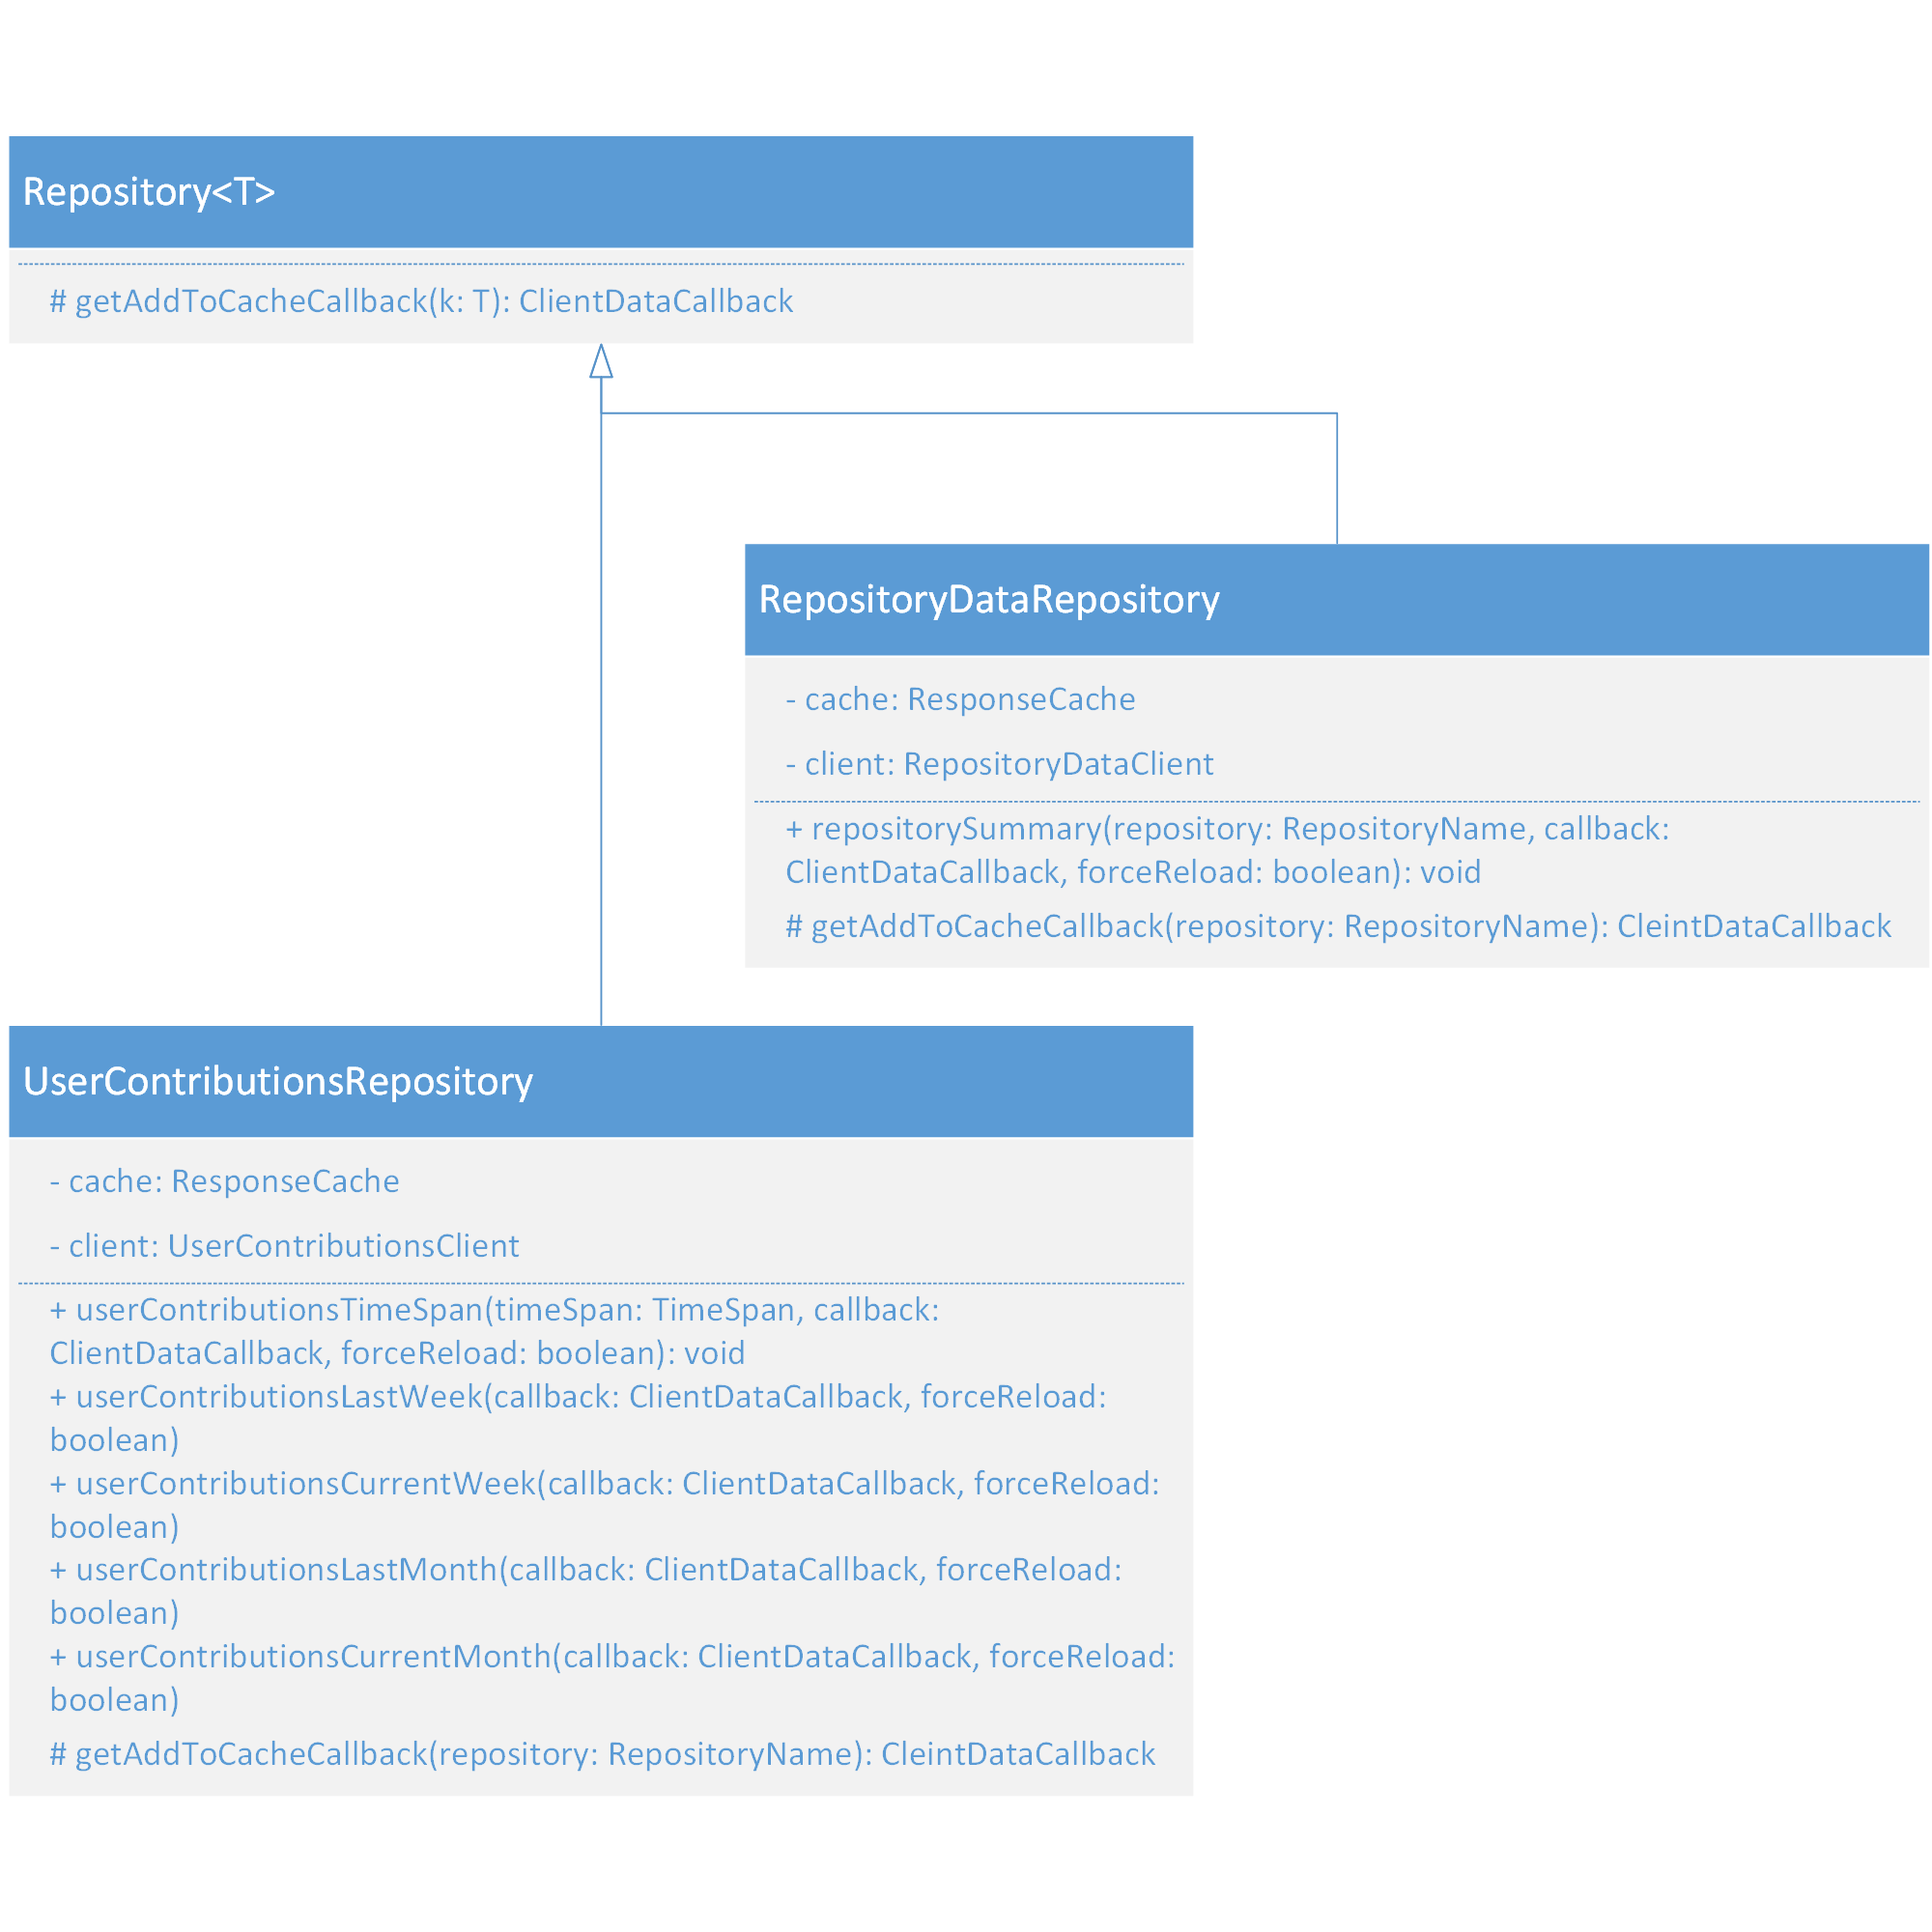
\includegraphics{refactoring_rename_method_repository_before.png}
  \centering
  \caption{UML vor Refactoring}
  \label{fig:RenameMethod_Refactoring_Before}
\end{figure}

\newpage
\subsubsection{UML Nacher}
Abbildung \ref{fig:RenameMethod_Refactoring_After} zeigt das UML-Klassendiagramm nach der Umbenennung der Methoden in \textit{UserContributionsRepository} und \textit{RepositoryDataRepository}.
\begin{figure}[h]
  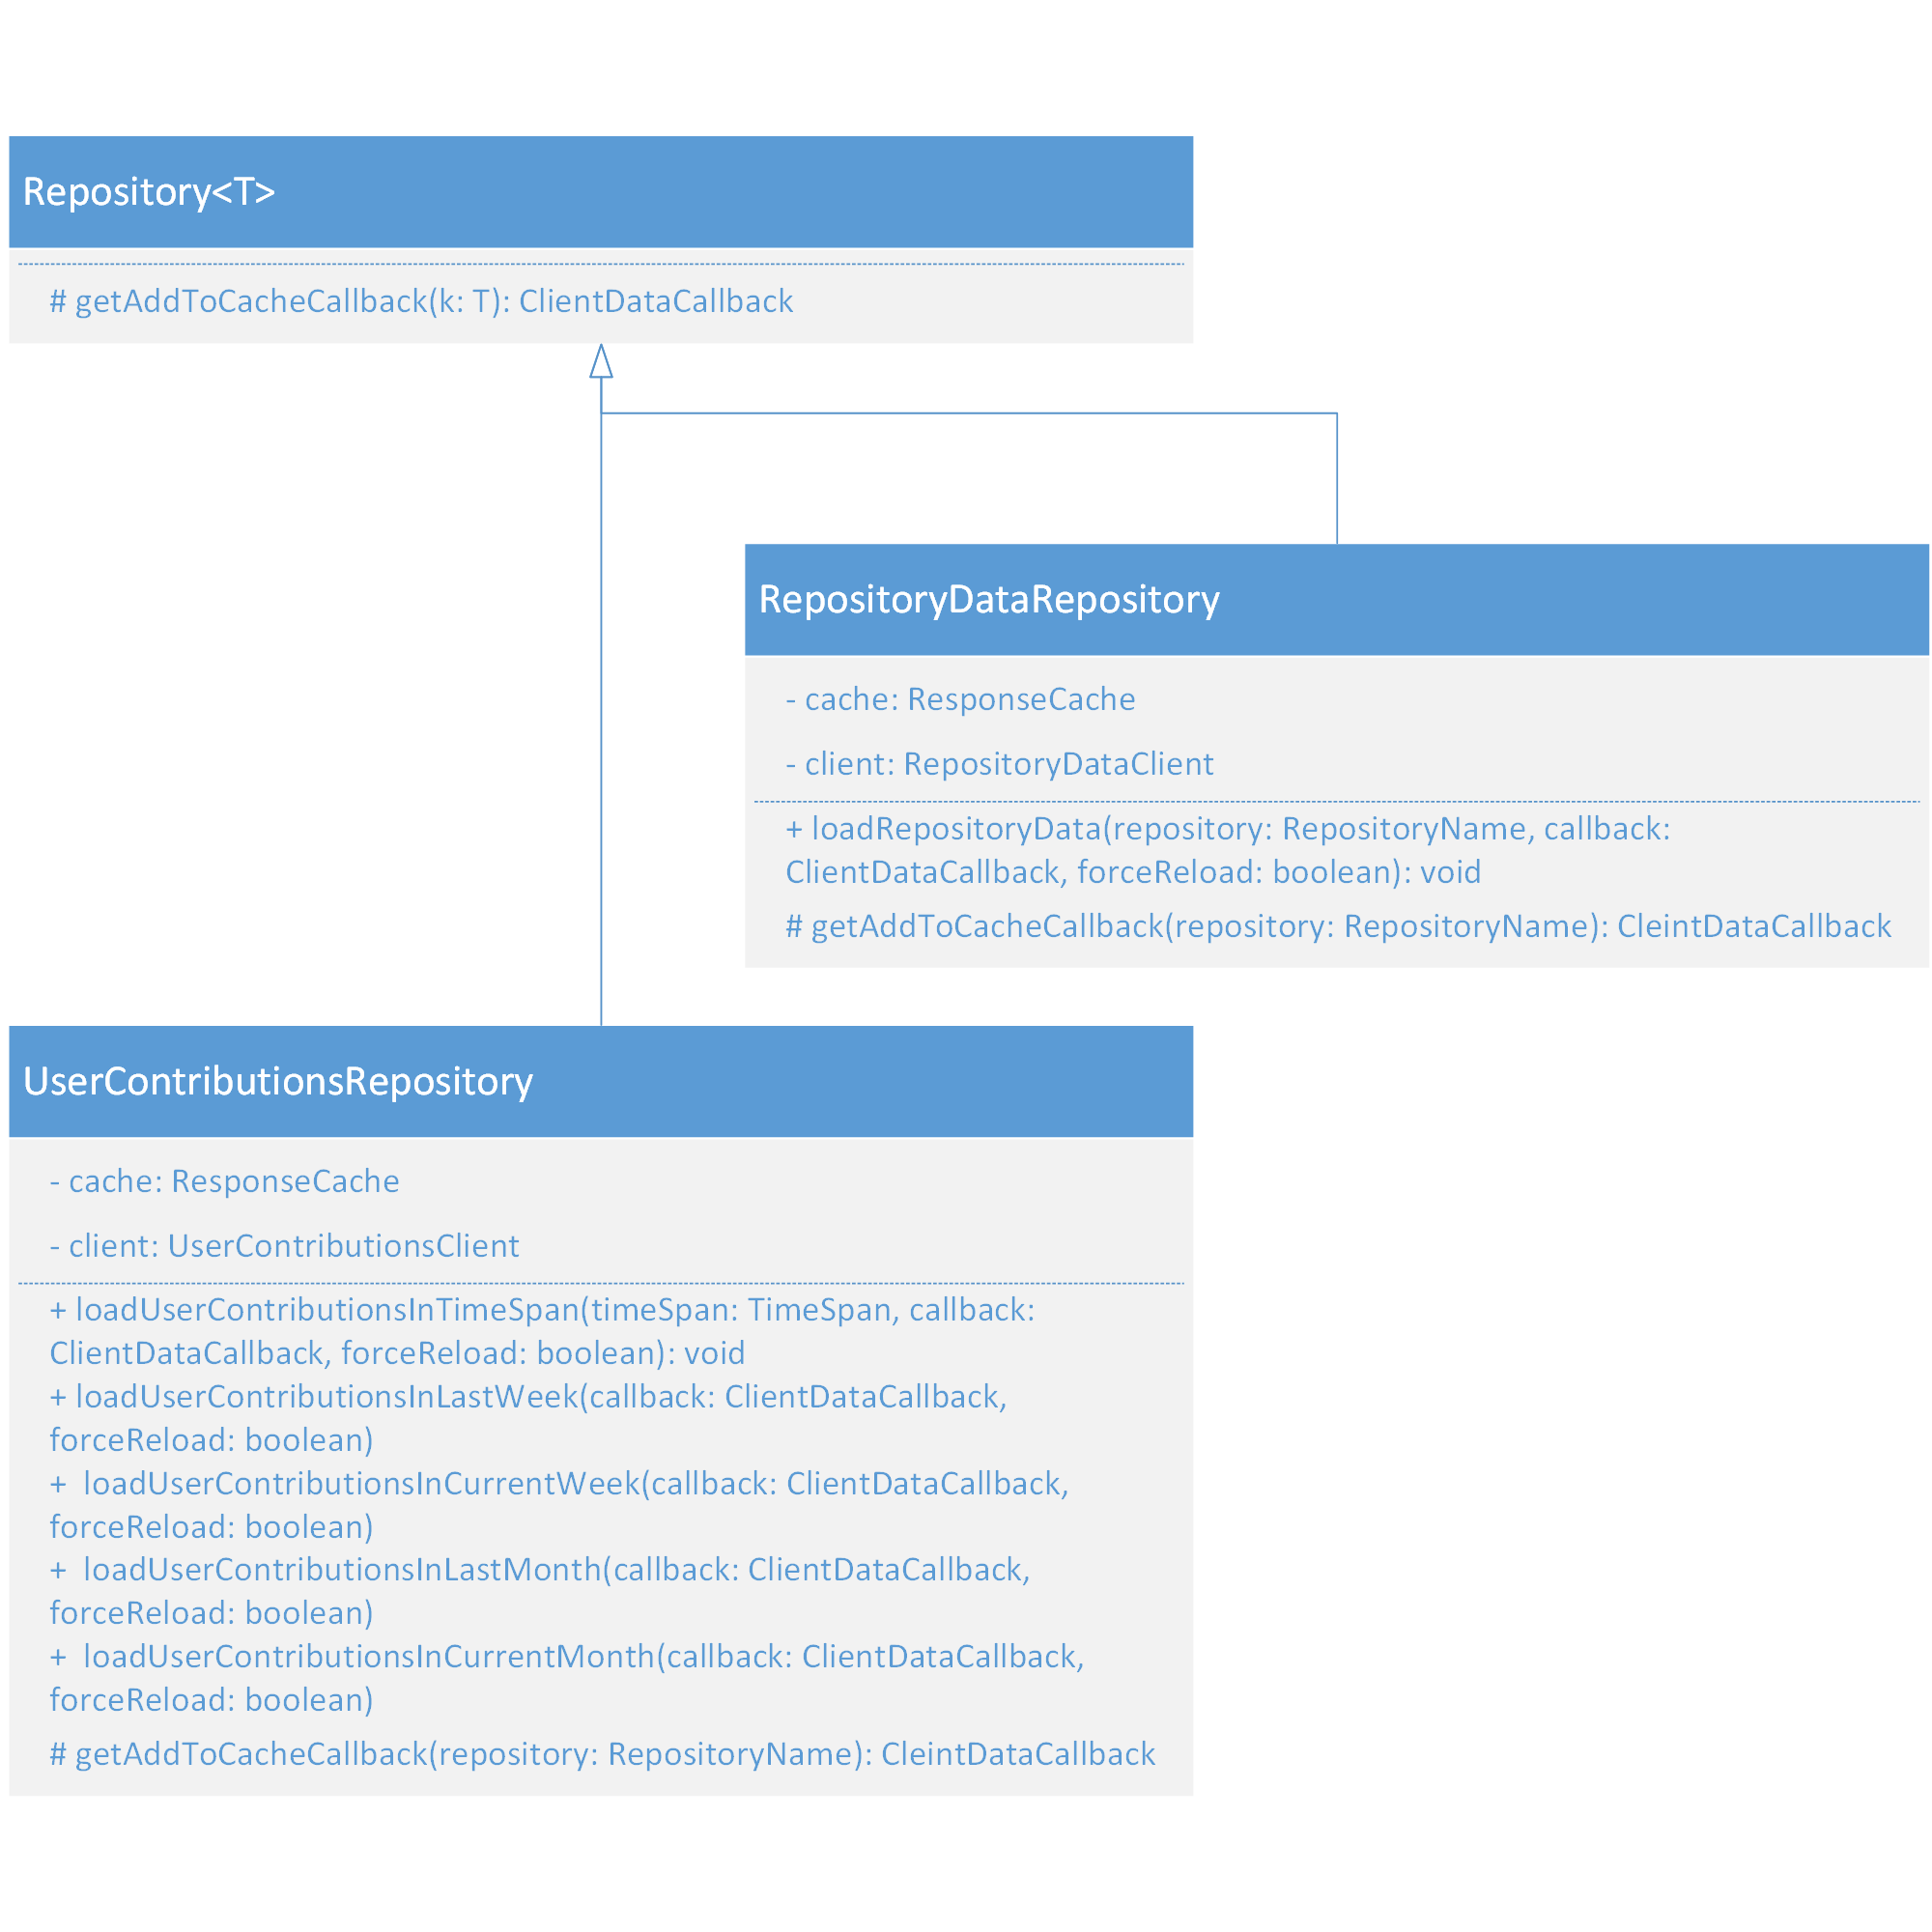
\includegraphics{refactoring_rename_method_repository_after.png}
  \caption{UML nach Refactoring}
  \label{fig:RenameMethod_Refactoring_After}
\end{figure}
\newpage

\chapter{Unit Testing}

\section{Analyse und Begründung für Umfang der Tests}

Um die Funktionalität der einzelnen Komponenten gewährleisten zu können werden Unit-Tests eingesetzt.
Dabei werden für die einzelnen Tests nur die, für diesen Test, relevanten Teile des Systems verwendet.
Da Abhängigkeiten zu anderen Komponenten die Tests nicht beeinflussen sollen werden alle anderen Komponenten durch Fake-/Mock-Objekte ersetzt.
Das Zusammenspiel mit den anderen Komponenten kann in Integrationstests getestet werden.
Außerdem tragen Unit-Tests auch zur Dokumentation bei, indem das gewünschte Verhalten der Komponente für Regel- und Ausnahmefälle in den Testfällen dokumentiert ist.
\newline
Für dieses Projekt wird \textit{JUnit} als Framework für die Erstellung und Ausführung von Java-Unit-Tests verwendet.
Bei der Implementierung der Tests wurde darauf geachtet die ATRIP-Regeln (\textit{Automatic, Thorough, Repeatable, Independent, Professional}) möglichst zu beachten.
\newline
Teile des Codes in diesem Projekt werden für Android-Spezifische UI-Aufgaben benötigt und können deshalb nur schlecht getestet werden. Das führt auch dazu, dass die Code-Coverage über das gesamte Projekt vergleichsweise klein sein kann und in diesem Fall keine sinnvolle Aussage über die Genauigkeit der Tests ermöglicht.
Stattdessen sollte hier zur Beurteilung der Testabdeckung nur die Code-Coverage der nicht-UI-Klassen betrachtet werden.
\newline
Allgemein wird darauf verzichtet triviale Funktionen, wie zum Beispiel Getter zu testen.
Tests dieser Funktionen würden bei großem Aufwand nur einen minimalen Mehrwert bringen, da keine "echte" Funktionalität getestet wird.
Stattdessen sollen sich die Tests auf relevante Funktionalität des Systems fokussieren.
Das bedeutet, dass vor allem die Klassen getestet werden sollen, die häufig verwendet werden und auch die Klassen, die für die Funktion der Anwendung unerlässlich sind.
UI-Klassen, die aufgrund starker Abhängigkeiten zu Android-Klassen schwer testbar sind sollen weniger ausführlich getestet werden.
\newline
Für die Tests innerhalb dieses Systems wurden drei Kernfunktionalitäten identifiziert, die von einer hohen Testabdeckung am stärksten profitieren.
Diese sind das Abrufen von Daten von der API, die Konvertierung von API-Datentypen zu Datentypen der Anwendung und in diesem Zusammenhang auch das Caching von abgerufenen Daten um die Netzwerklast zu reduzieren.
\newline
Diese Funktionalitäten verteilen sich auf die Packages \textit{analysis}, \textit{auth}, \textit{client}, \textit{data} und \textit{repository}.
Abbildung \hyperref{fig:Code_Coverage} zeigt einen Code-Coverage-Report dieser Packages (Stand: Commit \href{https://github.com/lukaspanni/OpenSourceStats/tree/28770def85a66a72b343e6640f2dbfa8ba073782}{28770de}).
Sten Pittet beschreibt in \cite{pittet_coverage}, dass 80\% Code-Coverage als gutes Ziel anerkannt sind, weshalb auch hier das Ziel gesetzt wird, mindestens 80\% der Methoden zu testen.
\begin{figure}[h]
  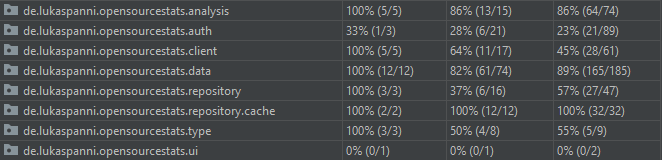
\includegraphics{Code_Coverage.png}
  \centering
  \caption{Code Coverage Report}
  \label{fig:Code_Coverage}
\end{figure}
Der Code-Coverage-Report, zeigt, dass alle relevanten Klassen getestet wurden.
Allerdings fällt dabei zunächst auf, dass die Coverage des \textit{ui}-Packages sehr schlecht ist, da der Fokus auf Tests der Funktionalität und nicht der Darstellung gelegt wurde.
Außerdem schwankt die Methoden-Coverage stark, was darauf zurückzuführen ist, dass versucht wurde, triviale Funktionalität nicht ausführlich zu testen.
Im Folgenden werden Funktionalität und Tests der einzelnen Packages noch weiter erläutert.
\newline
\newline
Das analysis-Package enthält alle Klassen, die für die Erstellung von Analysen verwendet werden.
Da diese Funktionalität, vermutlich noch am stärksten weiterentwickelt wird, wird hier eine gute Code-Coverage als sehr wichtig betrachtet.
Sowohl auf Methoden als auch auf Zeilen bezogen wird hier eine gute Code-Coverage von 86\% erreicht.
\newline
\newline
Im auth-Package, das alle Klassen die zur Authentifizierung benötigt werden enthält, wurde nur eine vergleichsweise kleine Code-Coverage von gerade mal 28\% aller Methoden erreicht, was als schlecht zu bewerten ist.
Da für die Authentifizierung eine Third-Party-Library verwendet wird, ist hier allerdings nicht mit angemessenem Aufwand eine höhere Coverage erreichbar.
Deshalb wurde die Entscheidung getroffen, die schlechte Coverage zu akzeptieren.
\newline
\newline
Das data-Package enthält alle Klassen, die als Nutzdaten von der Anwendung verarbeitet werden.
Antworten, die von der API empfangen werden, werden in einem ersten Schritt in einen solchen Datentyp konvertiert.
Diese Konvertierungen werden in den Konstruktoren der Klassen durchgeführt. Ansonsten werden diese Klassen hauptsächlich zur Speicherung von Anwendungsdaten verwendet und enthalten nur vergleichsweise wenig weitere Funktionalität.
Da die Konvertierung von API-Datentyp in Anwendungsdatentyp sehr häufig verwendet wird und die Anwendungsdatentypen generell an vielen verschiedenen verwendet werden, sind hier  ausführliche Tests notwendig.
Der Fokus der Tests liegt dabei auf den Konstruktoren, die wenigen weiteren Funktionalitäten der Klassen sind weniger wichtig und meist trivial.
Die Code-Coverage von 82\% aller Methoden wird deshalb als gut angesehen, vor allem wenn die Line-Coverage von 89\% in die Betrachtung mit einbezogen wird.
\newline
\newline
Im repository-Package, sind einerseits Repository-Klassen enthalten, die den Zugriff auf Anwendungsdaten abstrahieren und dabei das Caching der Daten transparent machen.
Andererseits finden sich hier auch die Klassen, die für die Umsetzung des Cachings verwendet werden.
Die Repository-Klassen übernehmen die Funktion, die Daten aus dem Cache abzurufen, wenn diese dort vorhanden sind und ansonsten die Daten über Funktionalität, die im client-Package implementiert ist von der API-abzurufen.
Als zentrale Komponente, um auf Daten zuzugreifen sind die Repository-Klassen deshalb  entscheidend für die Funktionalität der gesamten Anwendung.
Aus diesem Grund ist es wichtig hier eine möglichst hohe Testabdeckung zu erreichen.
Die niedrige Method-Coverage von nur 37\% ist hier trotzdem angemessen, da sie auf nicht getestete triviale Funktionen zurückzuführen ist.
Diese trivialen Funktionen sind verschieden Parametrisierte Konstruktoren und Hilfsfunktionen, die selbst wiederum nur Standard-Parameter für getestete Funktionen bereitstellen (siehe: \href{https://github.com/lukaspanni/OpenSourceStats/blob/ac3c4098d8f89f5eed7142d675ca49c4d3dd724f/app/src/main/java/de/lukaspanni/opensourcestats/repository/UserContributionsRepository.java#L51-L65}{UserCotributionsRepository.load...})
\newline
Die Komponente zum Caching ist ebenfalls wichtig, da ohne funktionierendes Caching sehr viele Anfragen über das Netzwerk gesendet werden müssen, was nicht nur die Menge der übertragenen Daten unnötig erhöht, sondern auch die Reaktionszeit der Anwendung verschlechtert.
Deshalb ist  auch im cache-Package eine hohe Testabdeckung wünschenswert.
In diesem Package wird sowohl für Method- als auch Line-Coverage ein Wert von 100\% erreicht, was als sehr gut zu bewerten ist.
Durch diese hohe Coverage soll sichergestellt werden, dass möglichst wenige Fehler beim Caching auftreten können und alle anderen Komponenten den Cache mit hoher Sicherheit verwenden können.
\newline
\newline
Das client-Package enthält alle Klassen, die benötigt werden, um Daten von der API abrufen zu können und steht damit, wie auch das cache-Package, im Zusammenhang mit dem Datenzugriff über die Repository-Klassen.
Es ist offensichtlich, dass auch diese Funktionalität von großer Bedeutung für die Funktionalität der Anwendung ist, und deshalb auch in diesem Package eine möglichst hohe Testabdeckung angestrebt wird.
Method- und Line-Coverage sind hier mit 64\% beziehungsweise 45\% nicht als gut zu bewerten.
Hier sollte die Coverage durch weitere Testes erhöht werden, was sich allerdings als schwierig herausstellte, da eine starke Kopplung an eine Thirt-Party-Library besteht, die nur schwer aufgelöst werden kann.
Deshalb wird die Code-Coverage aktuelle akzeptiert, sollte in Zukunft aber noch deutlich ausgebaut werden.
\newline
\newline
Im Screenshot ist zusätzlich das Package \textit{type} aufgeführt.
Dieses enthält ausschließlich automatisch generierten Java-Code, der für die Verwendung bestimmter Typen in Verbindung mit der GitHub-GraphQL-API benötigt wird.
Die Code-Coverage dieses Packages ist deshalb nicht relevant.
\newline
\newline
Im Gegensatz zu den genannten Bereichen ist eine hohe Testabdeckung im \textit{ui}-Package weniger wichtig und bringt nur wenig Nutzen. 
Zusätzlich ist hier aufgrund der genannten Einschränkungen eine hohe Testabdeckung nur mit sehr hohem Aufwand möglich.
Im Anbetracht des geringen Nutzens ist der Aufwand hier eine hohe Testabdeckung zu erreichen nicht gerechtfertigt, weshalb hier weitestgehend auf Tests verzichtet wird.

\newpage
\section{Analyse und Begründung für Einsatz von Fake-/Mock-Objekten}

Fake- und Mock-Objekte werden benötigt, um Abhängigkeiten einer Komponente zu anderen Komponenten in Unit-Tests zu reduzieren.
Sie implementieren dafür zum Beispiel das benötigte Interface, aber davon nur die aktuell benötigte Funktionalität.
Fake- und auch Mock-Objekte wurden eingesetzt, um Abhängigkeiten zu Third-Party-Komponenten, z.B. Android-Spezifische Klassen, und zu eigenen Klassen zu ersetzen.
Alle Fake- und Mock-Objekte sind im Package \textit{\href{https://github.com/lukaspanni/OpenSourceStats/tree/main/app/src/test/java/de/lukaspanni/opensourcestats/mock}{mock}} gesammelt.
\newline
Im Folgenden sollen beispielhaft einige der Fake-/Mock-Klassen genauer erläutert werden.
\newpage
\subsection*{\href{https://github.com/lukaspanni/OpenSourceStats/blob/main/app/src/test/java/de/lukaspanni/opensourcestats/mock/FakeUserContributionsClient.java}{FakeUserContributionsClient}}
Diese Klasse ist ein Fake-Objekt, das das Interface \textit{UserContributionsClient} implementiert. Diese Interface wir außerhalb der Tests für Clients verwendet, die bestimmte Daten (spezifisch: Objekte der Klasse \textit{UserContributionsResponse}) von einer API abrufen.
\newline
Offensichtlich sollen Tests von Klassen, die das Interface verwenden, auch ohne echte API-Anfragen möglich sein, da so auch weitere unerwünschte Abhängigkeiten im Test reduziert werden können. Die Klasse  \textit{FakeUserContributionsClient} implementiert dazu die Funktionen des Interfaces und zeichnet die Parameter der Methodenaufrufe auf, sodass Auswertungen im Test möglich sind.
\newline
Listing \ref{lst:FakeUserContributionsClient} zeigt beispielhaft, wie die Klasse \textit{FakeUserContributionsClient} im Rahmen eines Tests eingesetzt werden kann. Das Code-Beispiel stammt aus \href{https://github.com/lukaspanni/OpenSourceStats/blob/eafe840d0bfc8a08beca01709003d5afe7e59963/app/src/test/java/de/lukaspanni/opensourcestats/UserContributionsRepositoryUnitTest.java#L33-L47}{UserContributionsRepositoryUnitTest}.
\begin{lstlisting}[caption={Beispielhafte Verwendung von FakeUserContributionsClient}, label={lst:FakeUserContributionsClient}, captionpos={b}]
@Test
public void test_repository_summary_force_reload_client_not_cache() {
    TimeSpan timeSpan = TimeSpanFactory.getCurrentWeek();
    FakeUserContributionsClient client = new FakeUserContributionsClient();
    ResponseCache<TimeSpan, UserContributionsResponse> cache = new ResponseCache<>();
    UserContributionsRepository testObject = new UserContributionsRepository(cache, client);

    testObject.loadUserContributionsInTimeSpan(timeSpan, response -> {
    }, true);

    assertThat(client.isCalled(), is(true));
    //if hits or misses > 0 repository has tried to retrieve from cache
    assertThat(cache.getMisses(), is(equalTo(0)));
    assertThat(cache.getHits(), is(equalTo(0)));
}
\end{lstlisting}
In diesem Beispiel soll getestet werden, dass eine Instanz der Klasse \textit{UserContributionsRepository} bei setzen des Parameters forceReload die Daten nicht aus dem Cache bezieht sondern einen UserContributionsClient verwendet.
Um zu testen, ob eine Methode des UserContributionClient aufgerufen wird, wird in diesem Fall ein Objekt der Klasse \textit{FakeUserContributionsClient} als Implementierung von UserContributionClient an die Repository-Instanz übergeben. Nach dem Aufruf der Methode \textit{loadUserContributionsInTimeSpan} der Repository-Klasse wird geprüft, ob das Fake-Objekt einen Aufruf der Methode aufgezeichnet hat und ob Methoden des Caches aufgerufen wurden.
Wenn das Fake-Objekt aufgerufen wurde und der Cache nicht, dann ist das Verhalten in diesem Fall korrekt.

\newpage
\subsection*{\href{https://github.com/lukaspanni/OpenSourceStats/blob/main/app/src/test/java/de/lukaspanni/opensourcestats/mock/FakeResponseData.java}{FakeRespnseData}}
Die Klasse \textit{FakeResponseData} ist abgeleitet von der abstrakten Klasse \textit{ResponseData}, die die Basisklasse für alle Daten darstellt, die von der API als Antwort empfangen werden. Eingebettet in ein Objekt der Klasse \textit{CacheEntry} werden \textit{ResponseData}-Objekte im internen Cache (Objekte der Klasse \textit{ResponseCache}) gespeichert.
\newline
Für Tests der Klasse \textit{ResponseCache} werden also \textit{CacheEntry}-Objekte benötigt, die selbst wiederum ein Objekt der Klasse \textit{ResponseData} benötigen.
Um diese Objekte für Tests erstellen zu können muss eine  konkrete Klasse von \textit{ResponseData} abgeleitet werden. \textit{FakeResponseData} übernimmt diese Funktion und implementiert die Speicherung eines einfachen Integer-Werts als Test-Datum und die \textit{equals}-Methode um die Gleichheit zu anderen Objekten feststellen zu können.
Diese Funktionalität ist für Tests ausreichend.
\newline
Listing \ref{lst:FakeResponseData} zeigt, wie Objekte der Klasse \textit{FakeResponseData} in \textit{ResponseCache}-Tests verwendet werden. Das Codebeispiel stammt aus \href{https://github.com/lukaspanni/OpenSourceStats/blob/d0f67e73e4692b70316216688b7f556f42ccc11e/app/src/test/java/de/lukaspanni/opensourcestats/ResponseCacheUnitTest.java#L20-L32}{ResponseCacheUnitTest}.
\begin{lstlisting}[caption={Beispielhafte Verwendung von FakeResponseData}, label={lst:FakeResponseData}, captionpos={b}]
@Test
public void cache_get_returnsCorrectEntry() {
    ResponseCache<TimeSpan, FakeResponseData> testCache = new ResponseCache<>();
    FakeResponseData testResponseDataCorrect = new FakeResponseData(42);
    FakeResponseData testResponseDataWrong = new FakeResponseData(51);
    TimeSpan correctTimeSpan = new TimeSpan(new Date(2020, 11, 9), new Date(2020, 11, 10));
    TimeSpan wrongTimeSpan = new TimeSpan(new Date(2020, 10, 1), new Date(2020, 10, 2));
    testCache.put(correctTimeSpan, testResponseDataCorrect);
    testCache.put(wrongTimeSpan, testResponseDataWrong);

    ResponseData cachedData = testCache.get(correctTimeSpan);
    assertThat(cachedData, is(testResponseDataCorrect));
}
\end{lstlisting}
Der hier gezeigte Test soll testen, ob der \textit{ResponseCache} bei mehreren enthaltenen Elementen, die zu einem Key (in Form eines \textit{TimeSpan}-Objekts) passenden Daten zurückgibt.
Dazu werden gleich zwei \textit{FakeResponseData}-Objekte erstellt und mit eigenen Keys im Cache gespeichert. Abschließend wird geprüft, ob ein aus dem Cache angefordertes \textit{FakeResponseData}-Objekt, korrekt ist.

\documentclass[12pt]{article}
\usepackage[ngerman]{babel}
\usepackage[utf8]{inputenc}
\usepackage[hidelinks]{hyperref}
\usepackage{inconsolata}
\usepackage{color}
\usepackage{enumitem}
\usepackage[a4paper, left=2.5cm, right=2.5cm, top=2.5cm]{geometry}
\usepackage[onehalfspacing]{setspace}


\definecolor{pblue}{rgb}{0.13,0.13,1}
\definecolor{pgreen}{rgb}{0,0.5,0}
\definecolor{pred}{rgb}{0.9,0,0}
\definecolor{pgrey}{rgb}{0.46,0.45,0.48}

\usepackage{listings}
\lstset{language=Java,
  showspaces=false,
  showtabs=false,
  breaklines=true,
  showstringspaces=false,
  breakatwhitespace=true,
  commentstyle=\color{pgreen},
  keywordstyle=\color{pblue},
  stringstyle=\color{pred},
  basicstyle=\ttfamily,
  moredelim=[il][\textcolor{pgrey}]{$$},
  moredelim=[is][\textcolor{pgrey}]{\%\%}{\%\%}
}

\title{Programming Principles}
\date{DHBW Karlsruhe\\ Vorlesung Advanced Software Engineering Semester 5/6}
\author{Lukas Panni \\ TINF18B5}
\begin{document}
\maketitle

\newpage

\tableofcontents

\newpage
\section{SOLID}


\newpage
\section{GRASP}


\end{document}

\documentclass[12pt]{article}
\usepackage[ngerman]{babel}
\usepackage[utf8]{inputenc}
\usepackage[hidelinks]{hyperref}
\usepackage{inconsolata}
\usepackage{color}
\usepackage{enumitem}
\usepackage[a4paper, left=2.5cm, right=2.5cm, top=2.5cm]{geometry}
\usepackage[onehalfspacing]{setspace}


\definecolor{pblue}{rgb}{0.13,0.13,1}
\definecolor{pgreen}{rgb}{0,0.5,0}
\definecolor{pred}{rgb}{0.9,0,0}
\definecolor{pgrey}{rgb}{0.46,0.45,0.48}

\usepackage{listings}
\lstset{language=Java,
  showspaces=false,
  showtabs=false,
  breaklines=true,
  showstringspaces=false,
  breakatwhitespace=true,
  commentstyle=\color{pgreen},
  keywordstyle=\color{pblue},
  stringstyle=\color{pred},
  basicstyle=\ttfamily,
  moredelim=[il][\textcolor{pgrey}]{$$},
  moredelim=[is][\textcolor{pgrey}]{\%\%}{\%\%}
}


\title{Domain Driven Design}
\date{DHBW Karlsruhe\\ Vorlesung Advanced Software Engineering Semester 5/6}
\author{Lukas Panni \\ TINF18B5}
\begin{document}
\maketitle

\newpage
\tableofcontents
\newpage

\section{Analyse der Ubiquitous Language}

Kern des \textit{Domain Driven Design} ist das gemeinsame Verständnis der Problemdomäne. Dies ist notwendig, um ein präzises Modell der Domäne erstellen zu können.
Um die Kommunikation zwischen Entwicklern und Domänenexperten zu ermöglichen wird die sogenannte \textbf{Ubiquitous  Language} verwendet.
Da weder Domänenexperten die Sprache der Entwickler, noch umgekehrt die Entwickler die Sprache der Domänenexperten verstehen ist die Ubiquitous Language als gemeinsame Sprache unerlässlich.
Diese wird von Entwicklern und Domänenexperten gleichermaßen verwendet, um Begriffe, Prozesse und Konzepte eindeutig zu bezeichnen.
Wenn die Ubiquitous Language korrekt eingesetzt wird werden in der Domäne und im Quellcode der Anwendung die gleichen Begriffe für die gleichen Konzepte verwendet.
So können Missverständnisse und Mehrdeutigkeiten sicher vermieden werden, was gerade bei komplexen Domänen den Softwareerstellungsprozess erleichtert.
Beim definieren der Ubiquitous Language sollte der Fokus auf die Begriffe und Konzepte der Kerndomäne gelegt werden.
Andere Bereiche der Domäne können auch weniger genau modelliert werden, damit der Aufwand angemessen bleibt.
\newline
\newline
Die Kerndomäne dieses Projekts ist die Übersicht über Beteiligungen (Contributions) an Öffentlichen Repositories auf der Plattform \textit{GitHub}.
Die Ubiquitous Language ist dabei vergleichsweise einfach zu definieren, da sich die Anwendung an Entwickler richtet, die in diesem Fall gleichzeitig auch Domänenexperten sind.
Trotzdem muss darauf geachtet werden, dass einheitliche Begriffe verwendet werden.
Da die Plattform GitHub eindeutige Begriffe für die Bezeichnung von verschiedenen, wichtigen Konzepten verwendet und kein Einfluss auf diese Bezeichnungen besteht, wurde entschieden diese Bezeichnungen möglichst zu verwenden. Dabei werden diese Bezeichnungen nicht nur im Code sondern auch im User-Interface eingesetzt.

\subsection*{Repository / Repositories}
Der Begriff Repository beschreibt in diesem Kontext ein Verzeichnis, das zur Ablage von z.B. Programmcode verwendet werden kann.
Dabei bietet ein Repository bei GitHub aber auch noch weitere Funktionen, die hier aufgrund der Fehlenden Relevanz für das System nicht genauer erläutert werden.
Das Verständnis eines Repositoriy als Verzeichnis zur Ablage von Daten ist ausreichend.
Der Begriff wird sowohl im Code als auch im User-Interface verwendet.
Beispiele für die Verwendung des Begriffs im Code finden sich in der Klasse \href{https://github.com/lukaspanni/OpenSourceStats/blob/main/app/src/main/java/de/lukaspanni/opensourcestats/data/RepositoryDataResponse.java}{\textit{RepositoryDataResponse}}, die Daten zu einem Repository speichert, die von der API abgerufen wurden und in der Klasse \href{https://github.com/lukaspanni/OpenSourceStats/blob/main/app/src/main/java/de/lukaspanni/opensourcestats/data/ContributionRepositories.java}{\textit{ContributionRepositories}}, die beschreibt, in welchen Repositories Contributions durchgeführt wurden.
\newline
Beim Begriff Repository existiert allerdings eine Doppeldeutigkeit, da der Begriff Repository innerhalb des Systems auch als Bezeichnung für Klassen, die das \textit{Repository-Pattern} implementieren verwendet wird. Das führt zum Beispiel zu der Mehrdeutigen Bezeichnung der Klasse \href{https://github.com/lukaspanni/OpenSourceStats/blob/main/app/src/main/java/de/lukaspanni/opensourcestats/repository/RepositoryDataRepository.java}{RepositoryDataRepository}. Diese Mehrdeutigkeit kann nur schwer beseitigt werden, da einerseits der Repository-Begriff aus der Domänensprache verwendet werden soll, andererseits aber auch Repository-Pattern-Klassen eindeutig gekennzeichnet werden sollen. Deshalb wird diese Mehrdeutigkeit akzeptiert und festgelegt, dass Klassen die das Repository-Pattern implementieren, den Begriff Repository am Ende des Klassennamens enthalten. Kommt der Begriff an anderen Stellen vor, kann mit hoher Wahrscheinlichkeit davon ausgegangen werden, dass ein Repository im Sinne der Domäne gemeint ist.

\subsection*{Contribution / Contributions}
\label{sec:Contributions}
Beteiligungen an Repositories werden auf GitHub als Contributions bezeichnet. 
Die API, die verwendet wird um Daten abzurufen, verwendet ebenfalls diese Bezeichnung. 
Folglich soll auch im Code diese Bezeichnung für das gleiche Konzept verwendet werden.
\newline
Der Begriff Contributions ist allerdings nur ein Sammelbegriff für vier weitere Konzepte, die von großer Bedeutung für die Ubiquitous Language der Problemdomäne sind.
Diese Konzepte sind \hyperref[sec:Commits]{\textit{Commits}}, \hyperref[sec:Issues]{\textit{Issues}}, \hyperref[sec:PullRequests]{\textit{Pull Requests}} und \hyperref[sec:PullRequestReviews]{\textit{Pull Request Reviews}}, und werden im Folgenden beschrieben.
Die jeweilige Anzahl in einem bestimmten Zeitraum lässt sich über die GitHub-API abrufen und ist innerhalb dieser Anwendung von hoher Relevanz, da aus diesen Daten verschiedene Statistiken erstellt und dem Nutzer angezeigt werden.
\subsubsection*{Commit / Commits}
\label{sec:Commits}
Ein Commit kann in diesem Kontext als Prozess vorgenommene Änderungen am Quellcode zu bestätigen verstanden werden.
Die Anzahl der Commits in einem bestimmten Zeitraum erfasst so, wie viele unterschiedliche Änderungen ein Nutzer in diesem Zeitraum auf GitHub öffentlich gemacht hat. 
\subsubsection*{Issue / Issues}
\label{sec:Issues}
Issues werden bei GitHub verwendet um Ideen, neue Features, Aufgaben und Bugs zentral zu verwalten und stellen die zweite Art der Contribution dar.
Die Anzahl der Issues beschreibt, wie viele neue Issues ein Nutzer in einem bestimmten Zeitraum erstellt hat.
Diese Beschreibung reicht für das Verständnis im Rahmen dieses Projekts aus.
\subsubsection*{Pull Request / Pull Requests}
\label{sec:PullRequests}
GitHub verwendet sogenannte Pull Requests um Änderungen Code aus einem Branch in einen anderen, z.B. den main-Branch, zu übernehmen.
Dabei bietet ein Pull Request die Möglichkeit weitere Tests oder auch ein Code-Review durchzuführen, bevor der Pull Request angenommen wird.
Damit stellen Pull Requests ein wichtiges Konzept dar, das die Kollaboration erleichtert.
Die Anzahl an Pull Requests beschreibt, wie viele Pull Requests eine Nutzer in einem bestimmen Zeitraum erstellt hat.
\subsubsection*{Pull Request Review / Pull Request Reviews}
\label{sec:PullRequestReviews}
Ein Pull Request Review beschreibt bei GitHub ein Code-Review im Rahmen eines Pull Requests.
Das Kommentieren von Änderungen eines anderen Nutzers, die dieser in Form eines Pull Requests einreicht, wird dabei als Pull Request Review gewertet.
Die Anzahl von Pull Request Reviews beschreibt, wie viele Code-Reviews von Pull Requests anderer Nutzer durchgeführt wurden.
\newline
\newline
Die Klasse \href{https://github.com/lukaspanni/OpenSourceStats/blob/main/app/src/main/java/de/lukaspanni/opensourcestats/data/ContributionCount.java}{\textit{ContributionCount}} ist ein Beispiel dafür, wie alle Bezeichnungen, die im Zusammenhang mit Contributions stehen, auch im Code verwendet werden. Dies wird in Listing \ref{lst:ContributionCount} nochmals verdeutlicht. Die Klasse ContributionCount hat je eine Instanzvariable für die Anzahl von Commits, Issues, Pull Requests und Pull Request Reviews und verwendet somit alle vorgestellten Bezeichnungen, die in der Domäne im Zusammenhang mit Contributions verwendet werden.
\begin{lstlisting}[caption={Auszug aus der Klasse ContributionCount}, captionpos=b, label={lst:ContributionCount}]
public final class ContributionCount {

    private final int commitCount;
    private final int issueCount;
    private final int pullRequestCount;
    private final int pullRequestReviewCount;

    public ContributionCount(int commits, int issues, int pullRequests, int pullRequestReviews) {
        this.commitCount = Math.max(commits, 0);
        this.issueCount = Math.max(issues, 0);
        this.pullRequestCount = Math.max(pullRequests, 0);
        this.pullRequestReviewCount = Math.max(pullRequestReviews, 0);
    }
[...]
}
\end{lstlisting}
Auch im User-Interface werden diese Bezeichnungen gemeinsam verwendet, wie zum Beispiel die UI-Klasse \href{https://github.com/lukaspanni/OpenSourceStats/blob/main/app/src/main/java/de/lukaspanni/opensourcestats/ui/custom_elements/card/OverviewCard.java}{\textit{OverviewCard}} zeigt, die ebenfalls all diese Bezeichnungen verwendet.
\newline
Generell sind diese Begriffe von großer Bedeutung für das System und werden deshalb noch an vielen weiteren Stellen verwendet.
Weitere Beispiele sind unter anderem die Klasse \href{https://github.com/lukaspanni/OpenSourceStats/blob/main/app/src/main/java/de/lukaspanni/opensourcestats/data/ContributionCountChange.java}{\textit{ContributionCountChange}}, die eine Veränderung der Contribution-Anzahl im Vergleich zu einem anderen Zeitraum beschreibt und die zugehörige UI-Klasse \href{https://github.com/lukaspanni/OpenSourceStats/blob/main/app/src/main/java/de/lukaspanni/opensourcestats/ui/custom_elements/card/ProgressCard.java}{\textit{ProgressCard}}.




\newpage

\section{Analyse und Begründung von Value Objects}

\newpage

\section{Analyse und Begründung Entities}

\newpage

\section{Analyse und Begründung von Aggregates}

\newpage

\section{Analyse und Begründung Repositories}


\end{document}

\end{document}